\documentclass{report}

%====================== PACKAGES ======================

% region: packages

%\usepackage{extsize}
\usepackage[english]{babel}
\usepackage[utf8x]{inputenc}
%pour gérer les positionnement d'images
\usepackage{float}
\usepackage{amsmath}
\usepackage{graphicx}
\usepackage[colorinlistoftodos]{todonotes}
\usepackage{url}
%pour les informations sur un document compilé en PDF et les liens externes / internes
% \usepackage[hidelinks,colorlinks,linkcolor=black,]{hyperref}
\usepackage[hidelinks]{hyperref}
%pour la mise en page des tableaux
\usepackage{array}
\usepackage{tabularx}
%pour utiliser \floatbarrier
%\usepackage{placeins}
%\usepackage{floatrow}
%espacement entre les lignes
\usepackage{setspace}
%modifier la mise en page de l'abstract
\usepackage{abstract}
%police et mise en page (marges) du document
\usepackage[T1]{fontenc}
\usepackage[top=2.5cm, bottom=2.5cm, left=2.5cm, right=2.5cm]{geometry}
%Pour les galerie d'images
% \usepackage{subfig}

% endregion: packages

%====================== PACKAGES PERSO ======================

% region: packages perso

\usepackage{lmodern} % autre police d'écriture qui supporte le scaling
\usepackage[noabbrev]{cleveref} % références croisées [noabbrev] pour éviter les abréviations
\usepackage{acro} % acronymes (voir ici : https://tex.stackexchange.com/questions/492175/how-to-generate-list-of-abbreviations-in-latex)
\usepackage{mathrsfs}  % pour les polices mathématiques ex: \mathscr{X}
\usepackage{dsfont,amsfonts} % pour les polices mathématiques ex: \mathds{X}
% \usepackage{subfig} % pour les sous figures
\usepackage{lipsum} % pour générer du texte aléatoire
\usepackage{booktabs} % pour les tableaux
\usepackage{multirow} % pour les tableaux
\usepackage{etoc} % pour les tables des matières par chapitres 
\usepackage{algorithm} % pour les algorithmes
\usepackage{algorithmic} % pour les algorithmes
\usepackage[justification=justified,format=plain,labelfont=bf,width=0.9\textwidth]{caption}
\usepackage{bibentry} % Pour ajouter des refs qui ne sont pas citée directement
\usepackage{bm} % pour les polices mathématiques ex: \mathbf{X}
\usepackage{amssymb} % symboles mathématiques suplémentaires (comme \varnothing)
\usepackage{amsthm} % pour les théorèmes et surtout les preuves (voir ici: https://stackoverflow.com/questions/1449370/latex-error-environment-proof-undefined)
\usepackage[square,numbers]{natbib} % pour citer les auteurs directement [DEUX REFS] (1):https://tex.stackexchange.com/questions/69379/how-do-i-cite-author-in-latex (2) https://www.overleaf.com/learn/latex/Bibliography_management_with_natbib
\usepackage[left,modulo]{lineno} % pour numéroter les lignes
\usepackage{etoolbox} % for the \patchcmd command
\usepackage{subcaption}% pour avoir des sous tables et les sous figures (remplace subfig)
\usepackage{xcolor} % to use colors, specially for acronyms 
\usepackage{sectsty} % pour le style des sections (voir ici : https://tex.stackexchange.com/questions/311487/how-to-change-the-title-abstract-and-headings-font-to-sans-serif)
\usepackage{bbold} % pour les 1 avec 2 barres
\usepackage{stmaryrd} % pour les crochets d'intervalles

% endregion: packages perso


%====================== COMMANDES PERSO ======================
\newcommand\myfunc[5]{%
  \begingroup
  \setlength\arraycolsep{0pt}
  #1\colon\begin{array}[t]{c >{{}}c<{{}} c}
             #2 & \to & #3 \\ #4 & \mapsto & #5 
          \end{array}%
  \endgroup}

% Pour pouvoir créer des propotision (voir ici : https://www.overleaf.com/learn/latex/Theorems_and_proofs)
\newtheorem{proposition}{Proposition}[section]
\newtheorem*{remark}{Remark} % spécifique pour les remarques


% Patch abstract pour ne pas utiliser de "titlepage" et ainsi avoir une
% numérotation de page qui ne se remet pas à 1 à chaque chapitre.
% Voir ici : https://tex.stackexchange.com/a/483381
\patchcmd{\abstract}{\titlepage}{\cleardoublepage}{}{}
\patchcmd{\endabstract}{\endtitlepage}{\clearpage}{}{}
%====================== INFORMATION ET REGLES ======================

%rajouter les numérotation pour les \paragraphe et \subparagraphe
\setcounter{secnumdepth}{4}
\setcounter{tocdepth}{4}

% Réglage propres au document PDF

\hypersetup{							% Information sur le document
pdfauthor = {Robin Dupont},			% Auteurs
pdftitle = {Résumé du Manuscrit de Thèse de Robin Dupont},			% Titre du document
% pdfsubject = {Mémoire de Projet},		% Sujet
% pdfkeywords = {Tag1, Tag2, Tag3, ...},	% Mots-clefs
pdfstartview={FitH}}					% ajuste la page à la largueur de l'écran
%pdfcreator = {MikTeX},% Logiciel qui a crée le document
%pdfproducer = {}} % Société avec produit le logiciel


%====================== SECTION PERSO ====================== 
\DeclareAcronym{batch norm}{
  short=BN,
  long=Batch Normalisation,
}

\DeclareAcronym{CNN}{
  short=CNN,
  long=Convolutional Neural Network,
  long-plural=s,
}

\DeclareAcronym{GPU}{
    short=GPU,
    long=Graphics Processing Unit,
    long-plural=s,
}

\DeclareAcronym{amc}{
    short=AMC,
    long=AutoML for Model Compression,
}

\DeclareAcronym{nan}{
    short=\texttt{NaN},
    long=Not a Number,
}

\DeclareAcronym{FLOP}{
    short=FLOP,
    long=Floating Point Operation,
    long-plural=s,
}

\DeclareAcronym{ReLU}{
    short=ReLU,
    long=Rectified Linear Unit,
    long-plural=s,
}

\DeclareAcronym{STE}{
    short=STE,
    long=Straight Through Estimator,
}

\DeclareAcronym{LTH}{
    short=LTH,
    long=Lottery Ticket Hypothesis,
}

\DeclareAcronym{ASLP}{
    short=ASLP,
    long=Arbitrarily Shifted Log Parametrisation,
}

\DeclareAcronym{SGD}{
    short=SGD,
    long=Stochastic Gradient Descent,
}
\DeclareAcronym{LT}{
    short=LT,
    long=Lottery Ticket,
    long-plural=s,
}

\DeclareAcronym{GS}{
    short=GS,
    long=Gumbel-Softmax,
}

\DeclareAcronym{STGS}{
    short=STGS,
    long=Straight Through Gumbel-Softmax,
}

\DeclareAcronym{DWR}{
    short=DWR,
    long=Dynamic Weight Rescale,
}

\DeclareAcronym{SR}{
    short=SR,
    long=Smart Rescale,
}

\DeclareAcronym{WR}{
    short=WR,
    long=Weight Rescaling,
}

\DeclareAcronym{SC}{
    short=SC,
    long=Signed Constant,
}

\DeclareAcronym{FS}{
    short=FS,
    long=Fan Scaling,
}

\DeclareAcronym{NAS}{
    short=NAS,
    long=Neural Architecture Search,
}

\DeclareAcronym{KD}{
    short=KD,
    long=Knowledge Distillation,
}

\DeclareAcronym{MAC}{
    short=MAC,
    long=Multiply-Accumulate,
}

\DeclareAcronym{SE}{
    short=SE,
    long=Squeeze-and-Excitation,
}

\DeclareAcronym{FFT}{
    short=FFT,
    long=Fast Fourier Transform,
}

\DeclareAcronym{FPGA}{
    short=FPGA,
    long=Field Programmable Gate Array,
}

\DeclareAcronym{ANN}{
    short=ANN,
    long=Artificial Neural Network,
    long-plural=s,
}

\DeclareAcronym{DNN}{
    short=DNN,
    long=Deep Neural Network,
    long-plural=s,
}

\DeclareAcronym{MLP}{
    short=MLP,
    long=Multi-Layer Perceptron,
    long-plural=s,
}

\DeclareAcronym{FP32}{
    short=FP32,
    long=single-precision floating-point format,
}

\DeclareAcronym{PTQ}{
    short=PTQ,
    long=Post-Training Quantisation,
}

\DeclareAcronym{QAT}{
    short=QAT,
    long=Quantisation-Aware Training,
}

\DeclareAcronym{TA}{
    short=TA,
    long=Teacher Assistant,
    long-plural=s,
}
% ----- Hyphenation
% \hyphenation{re-para-me-tri-za-tion}
% \hyphenation{re-para-me-tri-sa-tion}
\hyphenation{der-nière}
\hyphenation{der-nières}
\hyphenation{der-nier}
\hyphenation{heu-ris-tique}
% ----- Style des liens
% \hypersetup{
%   citecolor=blue,
% }

% ################  A CHANGER POUR REVUE ?
\linespread{1} % régler l'espacement entre les lignes

\renewcommand\linenumberfont{\normalfont\large} % régler la taille des numéros de ligne

%======================== DEBUT DU DOCUMENT ========================

\begin{document}

% TODO: adapter pour le confort de lecture
\fontsize{14}{16}\selectfont

% style des sections : fonte sans serifs
\allsectionsfont{\sffamily}

%page de garde
% Original title page
% \title{\vspace{-3.0cm}Manuscript}
% \author{Robin Dupont}
% \date{}


\newcommand{\jurymember}[6]{\hspace{1.5em}{#6} \textbf{{#1} {#2}}, {#3}, {#4} \hfill \textit{{#5}}\\}

\newgeometry{left=2.8cm, right=2.5cm, top=2cm, bottom=2cm}
\begin{titlepage}

    \pdfbookmark[0]{Cover}{Cover}
    
    \begin{figure}
        \begin{subfigure}{.3\textwidth}
            \centering
            
\includegraphics[height=1.7cm]{title_page/assets/sorbonne.pdf}
        \end{subfigure}\hfill
        \begin{subfigure}{.3\textwidth}
            \centering
            
\includegraphics[height=1.7cm]{title_page/assets/LogoLIP6.pdf}
        \end{subfigure}\hfill
        \begin{subfigure}{.3\textwidth}
            \centering
            
\includegraphics[height=1.7cm]{title_page/assets/netatmo_logo_color.pdf}
        \end{subfigure}
    \end{figure}
    
    \begin{center}
        % {\large Thèse présentée pour l'obtention du grade de}\\
        {\large \textbf{THÈSE DE DOCTORAT DE SORBONNE UNIVERSITÉ}}\\
        \vspace{1em}
        {\large Spécialité - \textbf{Informatique}}\\
        \vspace{0.5em}
        {\large \textbf{Informatique, Télécommunication et Électronique (Paris) - ED130}}\\
    \end{center}
    \vfill
    \begin{center}
        \hfill
        \vfill
        {\Huge \textsf{Deep Neural Network Compression\\for Visual Recognition} }\\
        \vspace{1em}
        {\Large \textsf{Compression de Réseaux de Neurones Profonds\\pour la Reconnaissance Visuelle} }\\
        \vspace{2em}
        {\large Présentée par \par} 
        {\Large \textsf{Robin Dupont}\par}
        \vspace{2em}
        {\large Pour obtenir le grade de\par} 
        {\large \textbf{DOCTEUR de SORBONNE UNIVERSITÉ}}
        \vfill
    \end{center}
    \vspace{3em}
    \large
    %% TODO: If final version:
    Soutenue publiquement le 8 décembre 2023\\
    %% Else, for review version:
    % Version: \thesisVersion
    \begin{flushleft}
        Devant un jury composé de :\\
        \vspace{1em}
        \begin{tabularx}{\textwidth}{lXr}
            \textbf{Mme} & \begin{tabular}[t]{@{}l@{}}\textbf{Jenny Benois-Pineau} \\  Professeure, Université de Bordeaux \end{tabular}        & \textit{Rapportrice}            \\
            \textbf{M.}  & \begin{tabular}[t]{@{}l@{}}\textbf{Titus Bogdan Zaharia} \\ Professeur, Télécom SudParis\end{tabular}                & \textit{Rapporteur}             \\
            \textbf{M.}  & \begin{tabular}[t]{@{}l@{}}\textbf{Pierre Beauseroy} \\ Professeur, Université de Technologie de Troyes\end{tabular} & \textit{Examinateur}            \\
            \textbf{M.}  & \begin{tabular}[t]{@{}l@{}}\textbf{Nicolas Gac} \\ Professeur, Université Paris-Saclay\end{tabular}                  & \textit{Examinateur}            \\
            \textbf{M.}  & \begin{tabular}[t]{@{}l@{}}\textbf{Vincent Gripon} \\ Professeur, IMT Atlantique\end{tabular}                        & \textit{Examinateur}            \\
            \textbf{Mme} & \begin{tabular}[t]{@{}l@{}}\textbf{Alice Lebois} \\ Ingénieure, Netatmo\end{tabular}                                 & \textit{Co-encadrante de thèse} \\
            \textbf{M.}  & \begin{tabular}[t]{@{}l@{}}\textbf{Hichem Sahbi} \\ Chercheur CNRS (HDR), Sorbonne Université\end{tabular}           & \textit{Directeur de thèse}     \\
        \end{tabularx}

    \end{flushleft}
\end{titlepage}
\restoregeometry


%page blanche
%\newpage

%ne pas numéroter cette page
%\thispagestyle{empty}
%\newpage

%

% abstract

\begin{abstract}

    Thanks to the miniaturisation of electronics, embedded devices have become,
    more and more ubiquitous, since the 2010s, realising various tasks all
    around us. As their usage is developing, there is a growing demand for these
    devices to process data and make complex decisions efficiently. Deep neural
    networks are powerful tools to achieve this goal, however, these networks
    are often too heavy and complex to fit on embedded devices. Thus, there is a
    compelling need to devise methods to compress these large networks without
    significantly compromising their efficacy. This PhD thesis introduces two
    innovative methods, centred around the concept of pruning, aiming to
    compress neural networks while ensuring minimal impact on their accuracy.

    This PhD thesis first introduces a budget-aware method for compressing large
    neural networks with weight reparametrization and budget loss that does not
    require fine-tuning. Traditional pruning methods often rely on post-training
    saliency indicators to remove weights, disregarding the targeted pruning
    rate. Our approach integrates a budget loss, driving the pruning process
    towards a specific pruning rate during training, thereby achieving a joint
    optimisation of topology and weights. By soft-pruning the smallest weights
    using weight reparametrisation, our method significantly mitigates accuracy
    degradation in comparison to traditional pruning techniques. We show the
    effectiveness of our approach across various datasets and architectures.

    This PhD thesis later focuses on the extraction of effective subnetworks
    without weight training. Our goal is to identify the best subnetwork
    topology in a large network without optimising its weights while still
    delivering compelling performance. This is achieved using our novel
    Arbitrarily Shifted Log Parametrisation, which serves as a differentiable
    relaxation of discrete topology sampling, enabling the training of masks
    that represent the probability of selection of the weights. Alongside, a
    weight rescaling mechanism (referred to as Smart Rescale) is also
    introduced, which allows enhancing the performance of the extracted
    subnetworks and speeding up their training. Our proposed approach also finds
    the optimal pruning rate after one training pass, thereby circumventing
    computationally expensive gird-search and training across various pruning
    rates. As shown through comprehensive experiments, our method consistently
    outperforms state-of-the-art techniques and allows designing lightweight
    networks which can reach high sparsity levels without significant loss in
    accuracy.

\end{abstract}


\maketitle
% ----- Tables des matières, figures et tableaux  + acronymes ------
% \tableofcontents
% \listoffigures
% \listoftables
\newpage
% ---------------------------------------------------------------

\thispagestyle{empty}
\setcounter{page}{0}
%ne pas numéroter le sommaire

\newpage
% \printacronyms

%espacement entre les lignes d'un tableau
\renewcommand{\arraystretch}{1.5}

%====================== INCLUSION DES PARTIES ======================

~
\thispagestyle{empty}
%recommencer la numérotation des pages à "1"
\setcounter{page}{0}
\newpage

% ################  A CHANGER POUR REVUE ?
\linenumbers
\section*{Introduction}

La quatrième révolution industrielle, aussi appellée Industrie 4.0, a inauguré
l'intégration numérique des chaînes de production et des appareils intelligents
et connectés pour des systèmes de fabrication plus efficaces. En parallèle, la
recherche en intelligence artificielle a connu une croissance substantielle,
avec des avancées significatives en matière de systèmes d'apprentissage
automatique ou apprentissage machine.\\

Les réseaux de neurones profonds modernes offrent un potentiel significatif pour
renforcer les capacités des appareils connectés. Cependant, le déploiement  de
ces réseaux de neurones sur ces appareils présente un défi en raison de la
puissance de calcul et de l'espace mémoire limités. Pour palier à ce problème de
ressources, il est possible de déplacer les calculs vers le cloud, c'est à dire
vers de puissants serveurs distants. Cepdnant, traiter les données locatlement
présente des avantages: cela garantit une meilleure confidentialité des données,
limite les communications et par conséquent réduit la bande passante utilisée,
augmente la réactivité en réduisant la latence car il n'y a pas de transfers
réseau, et cela permet de construire des appareils capables de fonctionner en
autonomie.\\

Le travail de cette thèse CIFRE est réalisé dans le contexte industriel avec
Netatmo, une entreprise française spécialisée dans les appareils connectés
intelligents. Netatmo commercialise notamment des caméras d'interrieur et
d'extérieure capable d'effectuer de la détection d'objet de de la reconnaissance
faciale. Ces tâches sont réalisés directement sur la caméra afin de garantir la
confidentialité des données et de proposer des produits sans abonnements (les
coûts du cloud n'étant pas à couvrir). Netatmo utilise des réseaux de neurones
profonds pour ces tâches. Cependant, bien que performants, ces derniers sont
gourmands en ressources et ne peuvent pas être déployés tels quels sur les
caméras. Faire fonctionner ces réseaux de neurones directement sur les caméras
présente donc un cas convaincant pour le développement de réseaux de neurones
allégés, adaptés aux appareils connectés. Ces réseaux légers doivent atteindre
des niveaux de performance comparable à leurs homologues plus grands tout en
étant nettement moins gourmands en taille et en exigences de calcul.\\

Cette thèse aborde le défi de la compression des réseaux de neurones profonds à
travers l'élagage, une technique qui vise à réduire la taille d'un réseau de
neurones en supprimant les paramètres redondants ou inutiles. Elle présente en
particulier une méthode de reparametrisation des poids couplé à une fonction de
coût représentatn un budget qui permet d'éviter le réentrainement des poids
élagués, ainsi qu'une méthide de rééchantillonnage stochastique des poids qui ne
nécessitent pas d'entrainement des poids du réseau pour déterminer leur
pertinence au sein de l'architecture finale. Cela permet de rechercher une
topologie à la fois légère et performante à l'intérieur du réseau original sans
entrainer les poids.\\

\section*{Apprentissage profond et réseaux de neurones}

L'appentissage profond est un sous-domaine de l'apprentissage automatique qui se
concentre sur les réseaux de neurones profonds, un évolution des réseaux de
neurones artificiels. Ces derniers visent à apprendre une représentation des
données à partir d'informations non structurées telles que les images, le texte
ou l'audio. Ces réseaux ont été exploités dans diverses tâches, comme la
reconnaissance d'images et de parole, le traitement du langage naturel, la
détection d'objets entre autres
\cite{DBLP:conf/icml/AmodeiABCCCCCCD16,DBLP:conf/nips/RenHGS15,DBLP:conf/nips/KrizhevskySH12,
  DBLP:conf/emnlp/BudzianowskiV19,DBLP:conf/cvpr/HeZRS16,jumper2021highly}.
Historiquement, les réseaux de neurones artificiels ont cherché à reproduire les
réseaux neuronaux biologiques \cite{mcculloch1943logical} avant d'évoluer vers
des architectures plus complexes composées de blocs de base présentés dans la
suite.

\subsection*{Architectures Pionnières}\label{sec:dlo:early_architectures}

% Cette section présente le perceptron \cite{rosenblatt1958perceptron} et le
% \acl{MLP}, deux architectures fondamentales qui ont conduit au développement des
% \acp{DNN}.

Le premier modèle mathématique cherchant à reproduire le comportement d'un
neurone est le \emph{perceptron} \cite{rosenblatt1958perceptron}. Il s'agit d'un
modèle de neurone artificiel introduit par \citeauthor{rosenblatt1958perceptron}
qui est capable d'apprendre une limite de décision linéaire. Il est composé de
$n$ entrées $x_i$ pondérées par des poids $w_i$, qui sont ensuite passées par
une fonction d'activation non linéaire $g$. Sa formulation mathématique est
définie par l'équation \cref{eqn:dlo:perceptron}:

\begin{equation}
  \label{eqn:dlo:perceptron}
  \hat{y} = g(\sum_{i=1}^{n} w_i \cdot x_i + b)
\end{equation}

Une évolution directe du perceptron est le perceptron multi-couches qui est
composé de plusieurs couches de perceptrons aussi appelés neurones
\cite{rumelhart1986learning}. Il s'agit du type le plus simple de réseau de
neronnes artificiel. Une représentation du \ac{MLP} avec une couche cachée est
donnée dans \cref{fig:dlo:mlp}. Contrairement au perceptron, le perceptron
multicouche peut apprendre une frontière de décision non linéaire. Sa
formulation vectorielle est donnée par l'équation \cref{eqn:dlo:mlp}, où $g_i$
represente la fonction d'activation de la couche $i$, $\mathbf{w}_i$ les poids,
$\mathbf{b}_i$ le biais, et $\mathbf{x}$ l'entrée.

\begin{equation}
  \label{eqn:dlo:mlp}
  \hat{\mathbf{y}} = g_2(\mathbf{w}_2^T \cdot  g_1(\mathbf{w}_2^T \cdot \mathbf{x} + \mathbf{b}_1) + \mathbf{b}_2)
\end{equation}

\begin{figure}[htbp]
  \centering
  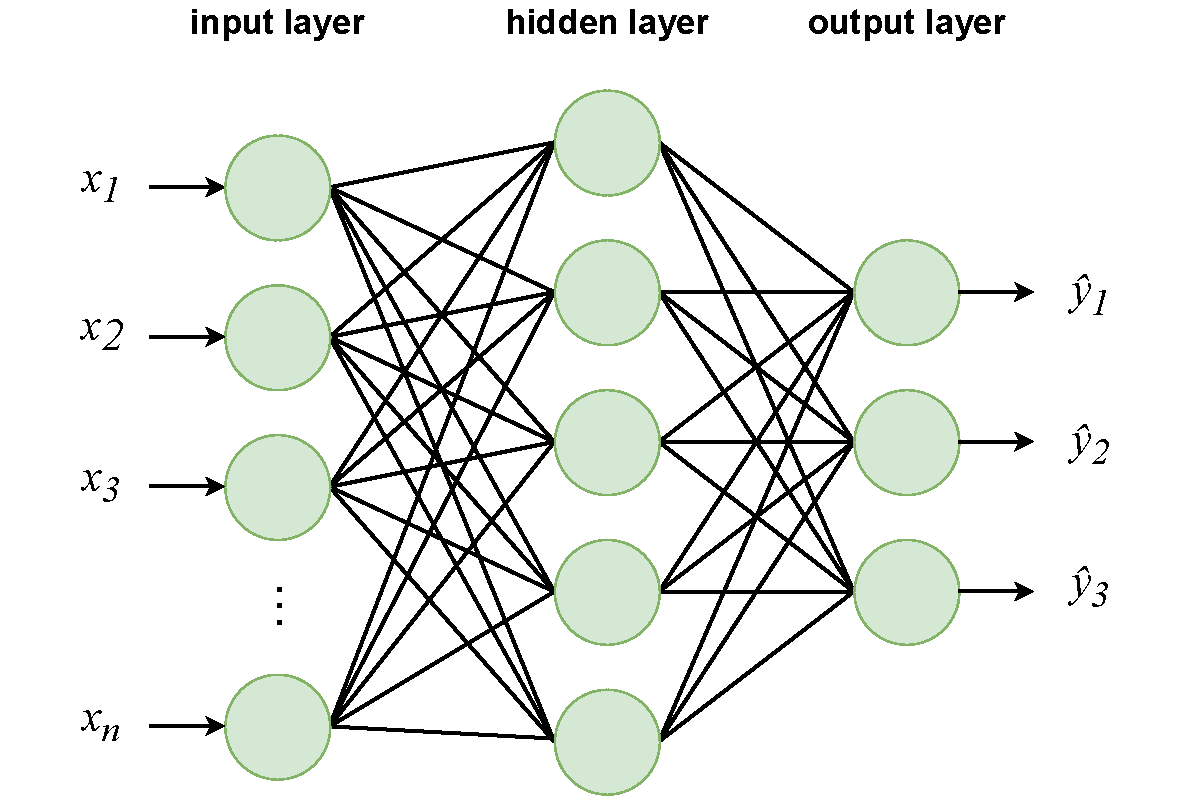
\includegraphics[width=0.5\textwidth]{./chapter_dlo/assets/mlp_scheme.pdf}
  \caption{Représentation d'un perceptron multi-couches avec une couche cachée.}
  \label{fig:dlo:mlp}
\end{figure}


\subsection*{Entrainement du réseau de neurones}\label{sec:dlo:training}

L'entraînement des réseaux neuronaux consiste en l'optimisation d'une fonction
de coût. Celle-ci quantifie la différence entre la sortie du réseau et la sortie
attendue. L'optimisation est faite en ajustant les paramètres du réseau,
également appelés poids et utilise principalement l'algorithme de
\emph{rétropropagation} \cite{rumelhart1986learning} pour calculer les gradients
et l'algorithme de descente de gradient stochastique
\cite{robbins1951stochastic} pour mettre à jour les poids.\\

Formellement, un réseau de neurones est une fonction de correspondance d'un
espace d'entrée $\mathcal{X}$ vers un espace de sortie $\mathcal{Y}$,
caractérisée par des paramètres $\theta$, appelés \emph{poids}. L'objectif est
d'ajuster $\theta$ pour que la sortie du réseau, $\hat{y}$, soit la plus proche
possible de la sortie réelle $y$ pour une entrée $X$ donnée. Dans le cas d'une
tâche de classification, la fonction de coût la plus courante est l'entropie
croisée qui s'écrie comme suit:

\begin{equation}
  \label{eqn:dlo:cross_entropy}
  \mathcal{L}_{\text{classif.}}(y, \hat{y}) = - \sum_{i=1}^{C} y_i \cdot \log(\hat{y}_i)
\end{equation}

\noindent où $C$ est le nombre de classes, $\mathcal{L}$ est la fonction de
coût, $y$ est la sortie attendue, aussi appelée \emph{vérité terrain}, et
$\hat{y}$ est la sortie prédite. Afin de réduire le risque de surapprentissage,
on adjoint à la fonction de coût une régularisation $\mathcal{R}(\theta)$ basée
sur les poids qui containt leur magnitude. $\mathcal{R}$ est généralement la
norme $\ell_1$ ou $\ell_2$ des poids. La fonction de coût finale est donc
$\mathcal{L} = \mathcal{L}_{\text{classif.}}(y,\hat{y}) +
  \mathcal{R}(\theta)$.\\


L'optimisation de cette fonction de coût est réalisée de manière itérative en
utilisant l'algorithme de descente de gradient stochastique. Cet algorithme
calcule le gradient de la fonction de coût par rapport aux paramètres du réseau
et met à jour les poids en fonction de ce gradient. La descente de gradient
stochastique est une variante de la descente de gradient classique qui calcule
le gradient sur l'ensemble des données d'entraînement. La descente de gradient
stochastique calcule le gradient sur un sous ensemble de données, appelé
mini-lot. Les poids sont mis à jour après chaque mini-lot de la manière
suivante :

\begin{equation}
  \label{eqn:dlo:sgd}
  \theta_{t+1} = \theta_t - \eta \cdot \nabla_{\theta_t} \mathcal{L}
\end{equation}

\noindent Ici, $\theta_t$ est le poids à l'itération $t$, $\eta$ est le taux
d'apprentissage qui contrôle la taille du pas de mise à jour des poids et
$\nabla_{\theta_t} \mathcal{L}$ est le gradient de la fonction de coût par
rapport aux paramètres du réseau. Ce dernier est calculé en utilisant le
théorème de dérivation des fonctions composées en tendem avec l'algorithme de
rétropropagation du gradient pour calculer le gradient de chaque poids de
manière efficace \cite{rumelhart1986learning}.\\

\subsection*{Architectures Convolutionnelles pour la Vision par Ordinateur}
Les Réseaux de neurones Convolutifs se sont imposés comme des architectures
performantes dans le domaine de la vision par ordinateur, notamment pour la
classification d'images. Leur efficacité réside dans leur capacité à apprendre
de manière hiérarchique des caractéristiques visuelles abstraites grâce aux
couches de convolution. Ils sont composé de différentes briques de bases
organisés en architectures. Ces briques de basent sont les suivantes:\\

\begin{itemize}
  \item \emph{Couche de convolution.} Cette couche effectue des convolutions
        spatiales sur les données d'entrée à l'aide de filtres, dont les poids sont
        entraînables, permettant d'extraire des caractéristiques allant d'un faible
        niveau d'abstraction (bords, coins, textures) à un haut niveau (objets,
        parties d'objets).
  \item \emph{Couche entièrement connectée.} Souvent situées à la fin des
        réseaux de neurones convolutifs, ces couches agissent comme des
        classificateurs. Elles réalisent des transformations non linéaires des
        caractéristiques extraites et se présente sous la forme de produits
        matriciels dont les vecteurs sont les caractéristiques extraites et les
        matrices les poids de la couche.
  \item \emph{Fonction d'activation.} Ces fonction, appliquées aux sorties des
        couches précédemment décrites, introduisent de la non-linéarité dans le
        réseau et permettent au modèle d'apprendre des motifs plus complexes. La
        fonction \ac{ReLU} ($\max(x,0)$) est la plus couramment utilisée. Elle
        présente les avantages d'être simple à calculer et de ne pas saturer
        pour des valeurs de sortie élevées. La sortie de cette couche est
        appelée l'\emph{activation}, en référence à l'activation biologique des
        neurones.
  \item \emph{Sous-échantillonnage (Pooling).} Cette couche réduit la dimension
        spatiale des représentations, diminuant ainsi le nombre de paramètres et les
        calculs dans les couches suivantes. Deux types courants sont le \emph{max
          pooling} et l'\emph{average pooling}. Le premier consiste à prendre la
        valeur maximale dans une fenêtre de taille $k \times k$ et le second à
        prendre la valeur moyenne.
  \item \emph{Normalisation par lot.} La normalisation par lot permet de lutter
        contre le changement de distribution entre les données d'entrainement et
        celles d'évaluation, accélérant ainsi l'entrainement et améliorant la
        généralisation. Elle est appliquée après les couches de convolution ou
        entièrement connectées et normalise les activations en utilisant la
        moyenne et l'écart-type de chaque mini-lot.
  \item \emph{Dropout.} Cette technique de régularisation permet d'éviter
        le surapprentissage. Elle désactive aléatoirement une proportion de neurones
        lors de chaque itération d'entrainement, poussant le réseau à apprendre des
        représentations plus robustes.
\end{itemize}

\subsection*{Architectures Modernes}

Les réseaux de neurones convolutifs profonds modernes ont connu plusieurs
évolutions qui ont conduit à des architectures plus profondes et plus
performantes, mais toujours composées des briques de bases présentées plus haut.
Un des premiers réseau de neurones convolutifs profonds est AlexNet
\cite{DBLP:conf/nips/KrizhevskySH12} qui comporte plusieurs couches de
convolutions suivies de couches entièrement connectées. VGG16
\cite{DBLP:journals/corr/SimonyanZ14a} est une évolution d'AlexNet qui comporte
d'avantage de couches de convolutions et des filtres de plus petite taille
($3\times 3$, contre $7 \times 7$ pour AlexNet), dont l'architecture est visible
sur la \cref{fig:dlo:vgg16}. ResNet \cite{DBLP:conf/cvpr/HeZRS16} est une
architecture plus récente qui comporte des connexions résiduelles entre les
couches. Ces connexions permettent de résoudre le problème de disparition du
gradient qui se produit lors de la rétropropagation dans les réseaux profonds.
La \cref{fig:dlo:resnet} présente l'architecture de ResNet-18. L'utilisation de
connexions résiduelles ont permis, entre autre, d'augmenter la profondeur des
réseaux de neurones (c'est à dire leur nombre de couches) ainsi que leurs
performances. En conséquence de ces avancées, les tailles des réseaux de
neronnes modernes sont maintenant trop importantes pour être déployés sur des
appareils connectés.\\

\begin{figure}
  \centering
  \subfloat[VGG16\label{fig:dlo:vgg16}]{
    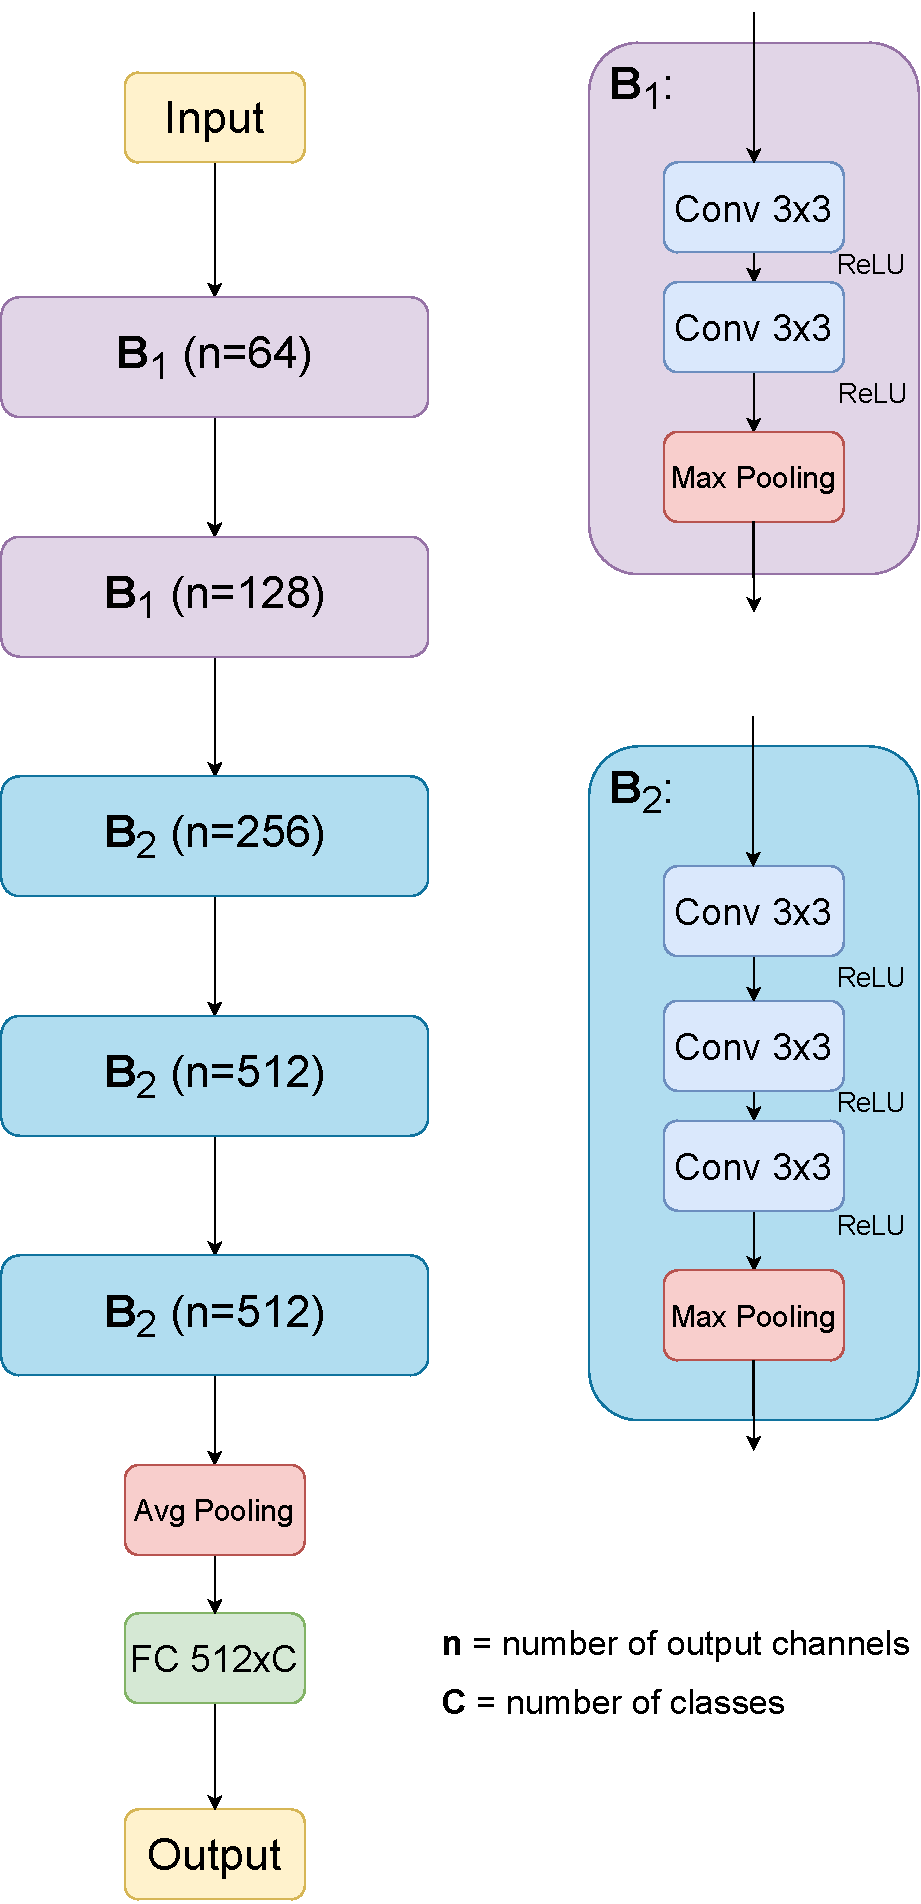
\includegraphics[width=0.3\textwidth]{./chapter_dlo/assets/vgg16_cifar.pdf}}
  \hspace{0.05\textwidth}
  \subfloat[ResNet-18\label{fig:dlo:resnet}]{
    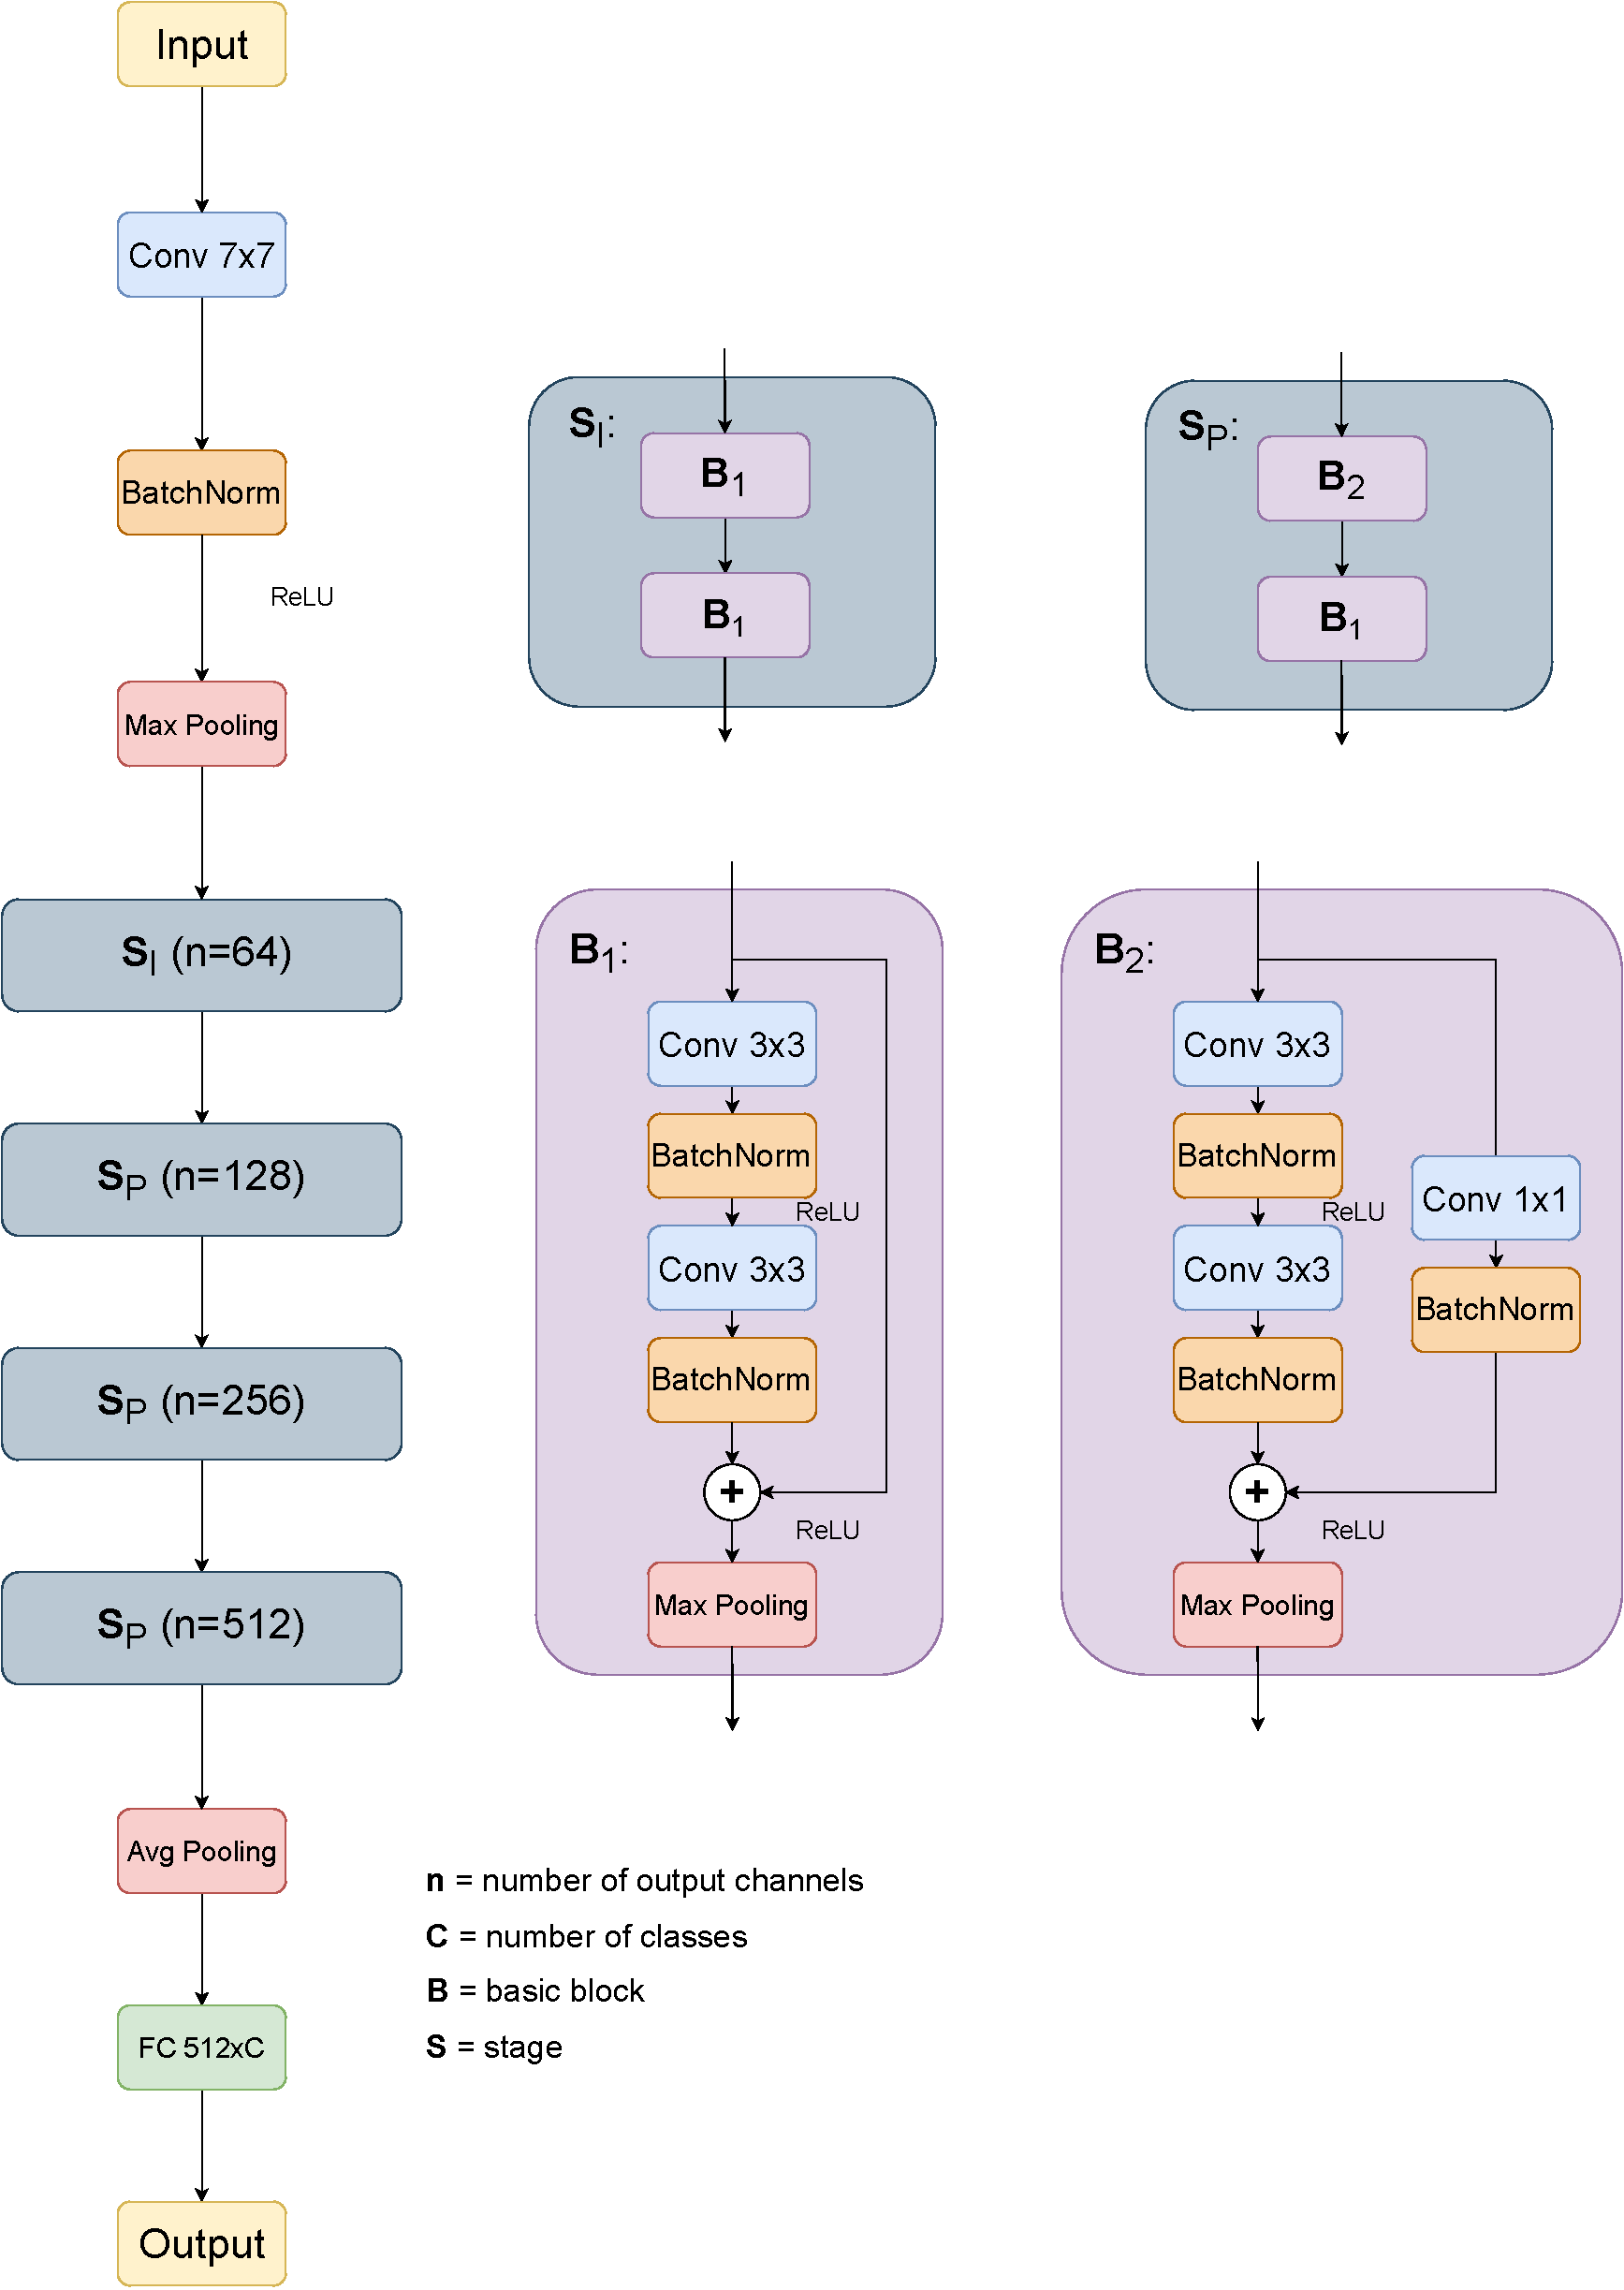
\includegraphics[width=0.5\textwidth]{./chapter_dlo/assets/resnet18.pdf}}
  \caption{Architecture de réseau de neurones convolutifs modernes.}
\end{figure}


\section*{Compression et accélération de réseaux de neurones}

Les réseaux de neurones profonds modernes comportent un nombre important de
couches et de paramètres, ce qui les rend gourmands en ressources. Cela pose un
problème pour leur déploiement sur des appareils qui ont des ressources
limitées. La compression des réseaux de neurones est une solution pour réduire
la taille des réseaux et les rendre plus légers. Elle permet également de
réduire les exigences de calcul et en mémoire, ce qui est particulièrement
important pour les appareils connectés, le stockage n'étant pas le facteur
limitant. La compression des réseaux de neurones n'est cependant pas sans
conséquence sur les performances. Celles-ci peuvent s'en retrouver dégréadées.
Les méthodes de compression et d'accélération peuvent êtres réparties en
plusieurs grandes familles de méthodes :\\

\noindent \textbf{Acceleration des opérations.} Les modèles de réseaux de
neurones convolutifs sont essentiellements composés d'opérations de convolution
et de multiplication matricielle. Dès lors, accélérer ces opérations permet un
gain en temps de calcul. Les opérations matricielles peuvent être accélérées en
de différente manières. En remarquant que l'opération de convolution dans le
domaine du problème $(y = x * k)$ est une multiplication dans le domaine de
Fourier $(y_{\mathcal{F}} = x_{\mathcal{F}} \times k_{\mathcal{F}})$, il est
possible d'accélérer les convolutions en utilisant la transformée de Fourier
inverse sur la multiplication des opérandes dans le domaine de Fourier $(y =
  \mathcal{F}^{-1} (x_{\mathcal{F}} \times k_{\mathcal{F}}))$
\cite{DBLP:conf/nips/ChiJM20,DBLP:journals/npl/LinY19,DBLP:conf/pkdd/PrattWCZ17}.
Il est également possible d'accélérer les multiplicatons matricielles en
optimisant directement l'ordre des opérations. C'est ce que propose de faire
l'algorithme de Strassen \cite{strassen1969gaussian}, plus tard almélioré dans
l'algorithme de Coppersmith-Winograd \cite{coppersmith1987matrix}. Ces
algorithmes décomposent récursivement une multiplication matricielle en
multiplications par blocs, qui sont ensuite réordonnés pour baisser le nombre
multiplication au prix d'un nombre d'addition accru (cependant, la complexité de
celles ci est négligeable devant celle des multiplications). On peut également
tirer parti des méthodes tout juste mentionnées pour accélérer les convolutions.
Pour ce faire, il faut transformer les opérations de convolution en
multiplication matricielle en représentant le noyeau de convolution comme une
matrice circulante \cite{DBLP:conf/iccv/ChengYFKCC15} ou une matrice de Toeplitz
\cite{gray2006toeplitz,liao2019compressing}.\\

\noindent \textbf{Paradigme Professeur-Élève.} Une des approches pour compresser
un réseau de neurones consiste à utiliser directement une petite achitecture et
a transférer les connaissances d'un réseau plus grand vers le plus petit. Le
petit réseau est alors appellé \emph{élève} et le grand réseau
\emph{professeur}. Ce procédé à été introduit par
\cite{DBLP:journals/corr/HintonVD15} \cite{DBLP:journals/corr/HintonVD15} qui
propose d'entrainer un petit réseau sur une tâche donnée et de rajouter dans à
la fonction de coût une régularisation basée sur la divergence de
Kullback-Leibler entre les sorties du petit réseau et celles du grand réseau,
également entrainé sur la même tâche. Cette régularisation permet de guider
l'élève vers les sorties du professeur. La fonction de coût totale s'écrit donc
:\\

\begin{equation}
  \mathcal{L}_{\text{totale}} = \underbrace{\mathcal{L}_{\text{CE}}(\hat{y}_{e}, y)\vphantom{\left(\frac{\hat{y}_{e}}{T}, \frac{\hat{y}_{p}}{T}\right)}}_{\text{Tâche}} +
  \lambda \frac{T^{2}}{2}\underbrace{\mathcal{L}_{\text{CE}}\left(\frac{\hat{y}_{e}}{T}, \frac{\hat{y}_{p}}{T}\right)}_{\text{Distillation}}
\end{equation}\\

\noindent où $\mathcal{L}_{\text{CE}}$ est l'entropie croisée (voir
\cref{eqn:dlo:cross_entropy}) et $\lambda\frac{T^{2}}{2}$ est un coefficient de
ponderation des 2 fonctions de coût. Cette méthode a inspiré d'autres approches
qui se basent sur le même principe : le transfer de connaissances d'un réseau à
un autre, mais en utilisant d'autres régularisations.
\citeauthor{DBLP:journals/corr/RomeroBKCGB14}
\cite{DBLP:journals/corr/RomeroBKCGB14} propose d'utiliser une norme $\ell_2$
pour quantifier l'écart des cartes d'activations entre le professeur et l'élève.
Cette méthode a été améliorée dans \cite{DBLP:conf/iclr/ZagoruykoK17} ou l'on
considère l'attention plutôt que les cartes d'activation pour transferer la
connaissance. La distillation telle que présentée dans
\cite{DBLP:journals/corr/HintonVD15} a été revisité dans
\cite{DBLP:conf/aaai/MirzadehFLLMG20}, qui propose de mettre en place un
\emph{assistant} qui est un réseau de taille intermédiaire entre l'élève et le
professeur afin de proposer une transition plus douce entre les 2 réseaux.
Enfin, une variante de l'approche professeur-élève a été présentée dans
\cite{DBLP:conf/cvpr/ZhangXHL18} où tous les réseaux sont à la fois élève et
professeur.\\


\noindent \textbf{Architecture spécifiques.} Afin de permettre le déploiement de
réseaux de neurones sur des appareils aux ressources limitées, des travaux de
recherche se sont employés à concevoir des architectures spécifiques basées sur
de nouvelles briques de bases qui permettent de réduire la taille des réseaux
tout en conservant leurs performances. MobileNet
\cite{DBLP:journals/corr/HowardZCKWWAA17} est le parfait exemple de ce type de
réseau. Il est composé de \emph{convolutions séparables en profondeurs} qui
permettent de réduire le nombre de paramètres et de calculs (voir
\cref{fig:dlo:depthwise_separable_conv}). Les convolutions séparables en
profondeurs sont composées de 2 opérations : une convolution \emph{en
  profondeur} et une convolution \emph{en largeur}. La convolution en profondeur
est une convolution spatiale classique, tandis que la convolution en largeur est
une convolution $1 \times 1$ qui permet de réduire le nombre de canaux. D'autres
briques de bases ont été proposées dans les achitectures SqueezeNet
\cite{DBLP:journals/corr/IandolaMAHDK16} et ShuffleNet
\cite{ZhangShuffleNet,MaShuffleNetV2}. Le premier introduit les \emph{fire
  modules} qui sont des couches de convolution qui mélangent différentes tailles
de noyeau de convolution, afin de préserver l'expressivité du réseau tout en
limitant le nombre de paramètres avec des noyeau plus petits. Le second propose
le concept de \emph{channel shuffle} couplé à des convolutions groupées, ce qui
permet de partager les caractéristiques apprises entre les groupes.\\

Si ces architectures sont performantes, elles ont été conçues à la main par des
humains et ont nécessité beaucoup de travail et d'expertise. Il est possible
d'obtenir d'autres architecture de manière automatique en utilisant des méthodes
de recherche d'architecture. Celles-ci sont basées sur des algorithmes
d'optimisation qui cherchent à trouver la meilleure architecture pour une tâche
donnée. Parmi ces méthodes, on peut citer les algorithmes génétiques
\cite{DBLP:conf/icml/RealMSSSTLK17} et les algorithmes de recherche bayésienne
\cite{DBLP:conf/nips/BergstraBBK11}. D'autres méthodes sont basées sur des
relaxations continue du problème et sont optimisées avec une descente de
gradient \cite{DBLP:conf/iclr/LiuSY19}.\\

\begin{figure}[htbp]
  \centering
  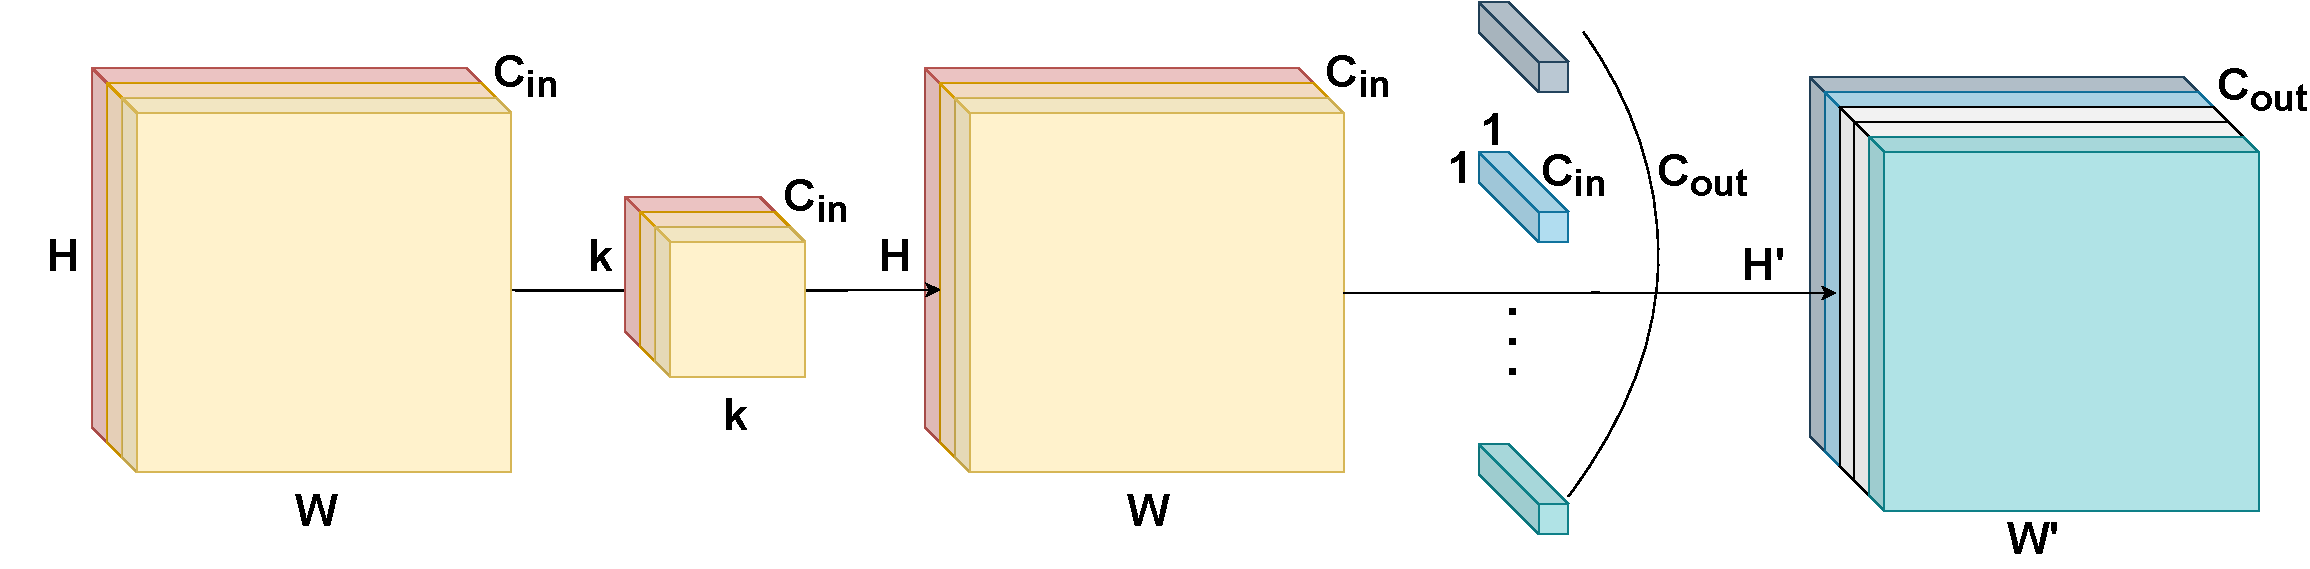
\includegraphics[width=0.7\textwidth]{./chapter_sota/assets/depthwise_sep_conv_scheme.pdf}
  \caption{Convolution séparables en profondeur.}
  \label{fig:dlo:depthwise_separable_conv}
\end{figure}

\noindent \textbf{Compression d'architectures existantes.} Les méthodes basée
sur la paradisme Professeur-Élève, les architectures spécifiques et celles
obtenues par recherche d'architecture  partagent toute la caractéristiques
suivante : la création d'un nouveau d'une achitecture spécifique qui répond à un
besoin donné. Cependant, il est également possible de compresser des des
architectures déjà existantes en les modifiant. C'est ce que propose les
méthodes de quantisation, binarisation et élagage.  La quantisation consiste à
réduire la précision des poids et des activations. Au lieu de traiter avec des
valeurs flottantes avec une précision de 32 bits, des représentations sur moins
de bits sont utilisées, avec par exemple des représentations sur 8 bits
\cite{37631} ou 16 bits \cite{gupta2015deep}. La quantisation peut également
être utilisée en combinaison avec un partionnement en K-moyennes
\cite{DBLP:journals/corr/HanMD15}. Les poids peuvent alors prendre $K$ valeurs
possibles, ces dernières étant les centroïdes du partitionnement. Cette approche
est utile pour la compression pure, mais contrairement à une approche de
quantisation classique qui réduit la précision de la représentation, cette
approche ne permet pas de gain en temps de calcul. La binarisation est une forme
extrême de quantisation où les poids sont représentés par des valeurs binaires
($+1$ ou $-1$) \cite{courbariaux2015binaryconnect}. D'autres travaux se sont
également intéressé à la binarisation des poids et des activations
\cite{DBLP:conf/nips/HubaraCSEB16}. La quantisation ou la binarisation peuvent
être effectuées après l'entrainement du réseau
\cite{tensorrt,DBLP:journals/corr/HanMD15} mais cela induit une perte en
performance. C'est pourquoi d'autres travaux se sont employés à quantifier les
réseaux de neurones pendant l'entrainement soit de manière effective
\cite{courbariaux2015binaryconnect,DBLP:conf/nips/HubaraCSEB16} soit en simulant
l'effet de la quantisation pendant l'entrainement
\cite{DBLP:conf/cvpr/JacobKCZTHAK18}.\\

L'élagage est une autre méthode de compression qui consiste à modifier un réseau
déjà existant en supprimant des poids jugés non importants ou redondants. On
peut classer les méthodes d'élagage en 2 grandes catégories en fonction de la
granularité avec laquelle les poids sont retirés. Ces 2 familles sont :
l'élagage structuré et l'élagage non structuré (voir \cref{fig:sota:pruning}).
L'élaguge structuré consiste en la suppression de structures entières du
réseau, le plus souvent des canaux de convolution entiers, mais également des
lignes et des colonnes de matrices de poids, des filtres de convolution entiers
ou même des sous parties du réseau. L'importance des ses structures est évaluée
de différentes manières et peut être soit basée sur la valeur même des poids qui
la compose \cite{DBLP:conf/iclr/0022KDSG17} soit sur des indicateurs qui en sont
directement dérivés \cite{DBLP:conf/cvpr/HeLWHY19,DBLP:conf/cvpr/WangLW21}.
D'autres travaux se concentrent sur les activations et proposent l'élagage de
des canneaux les plus redondants \cite{DBLP:conf/iccv/HeZS17} ou bien de ceux
qui contiennent le plus de valeurs nulles \cite{DBLP:journals/corr/HuPTT16}.
\cite{DBLP:conf/iccv/LiuLSHYZ17} et \cite{DBLP:conf/nips/YouYYM019} proposent
d'introduire des variables auxiliaires qui permettent de quantifier l'importance
de chaque canneaux et de les élaguer en conséquence. Ce concept est à la base de
divers travaux qui introduisent des méthodes d'élagage dynamiques qui
appliquent celui-ci pendant l'entrainement et non a posteriori
\cite{DBLP:conf/nips/GuoYC16,DBLP:conf/ijcai/HeKDFY18}.\\

La deuxième grande famille d'élagage est l'élagage non structuré. Cette famille
regroupe des méthodes qui se concentrent sur l'élagage individuel des poids.
Parmis les premières méthodes d'élagage non structuré, on peut citer les
méthodes basées sur la Hessienne de la fonction de coût
\cite{DBLP:conf/nips/CunDS89,DBLP:conf/icnn/HassibiSW93}. Ces approches
utilisent la Hessienne pour déterminer l'impact du retrait d'un poids sur la
fonction de coût et pour corriger les poids restants en conséquence. Du fait de
la complexité de calcul de la Hessienne, ces méthodes ne sont plus adaptés aux
architectures modernes. D'autres méthodes se sont intéressées à l'élagage non
structuré en utilisant des indicateurs basés sur la valeur (ou magnitude) des
poids \cite{DBLP:conf/nips/HanPTD15} et proposent de réentrainer les poids
restants de manière itérative. Ces travaux ont inspiré le concept de
\emph{Lottery Ticket} \cite{DBLP:journals/corr/abs-1903-01611}: un \emph{Lottery
  Ticket} (billet de lotterie) est un sous réseau de neurones qui, quand il est
entrainé indépendamment, atteint une précision équivalente à celle du réseau
complet dont il est extrait. Les \emph{Lottery Tickets} sont identifiés en
entrainant un réseau et en élaguant les poids les moins importants. Les poids du
sous réseau sont ensuite initialisés avec les poids originaux du réseau complet.
Cette découverte a été analysée dans \cite{DBLP:conf/nips/ZhouLLY19} et étendu à
des réseaux plus profonds dans \cite{DBLP:journals/corr/abs-1903-01611}.
L'existence du \emph{Lottery Ticket} (ou en d'autres termes le sous-réseau) a
été théoriquement prouvée dans \cite{DBLP:conf/icml/MalachYSS20} et les
exigences sur la taille théorique du réseau d'origine ont été affinées
ultérieurement \cite{DBLP:conf/nips/PensiaRNVP20,DBLP:conf/nips/OrseauHR20}.


\begin{figure}
  \centering
  \subfloat[Élagage structuré\label{fig:sota:structured_pruning}]{%
    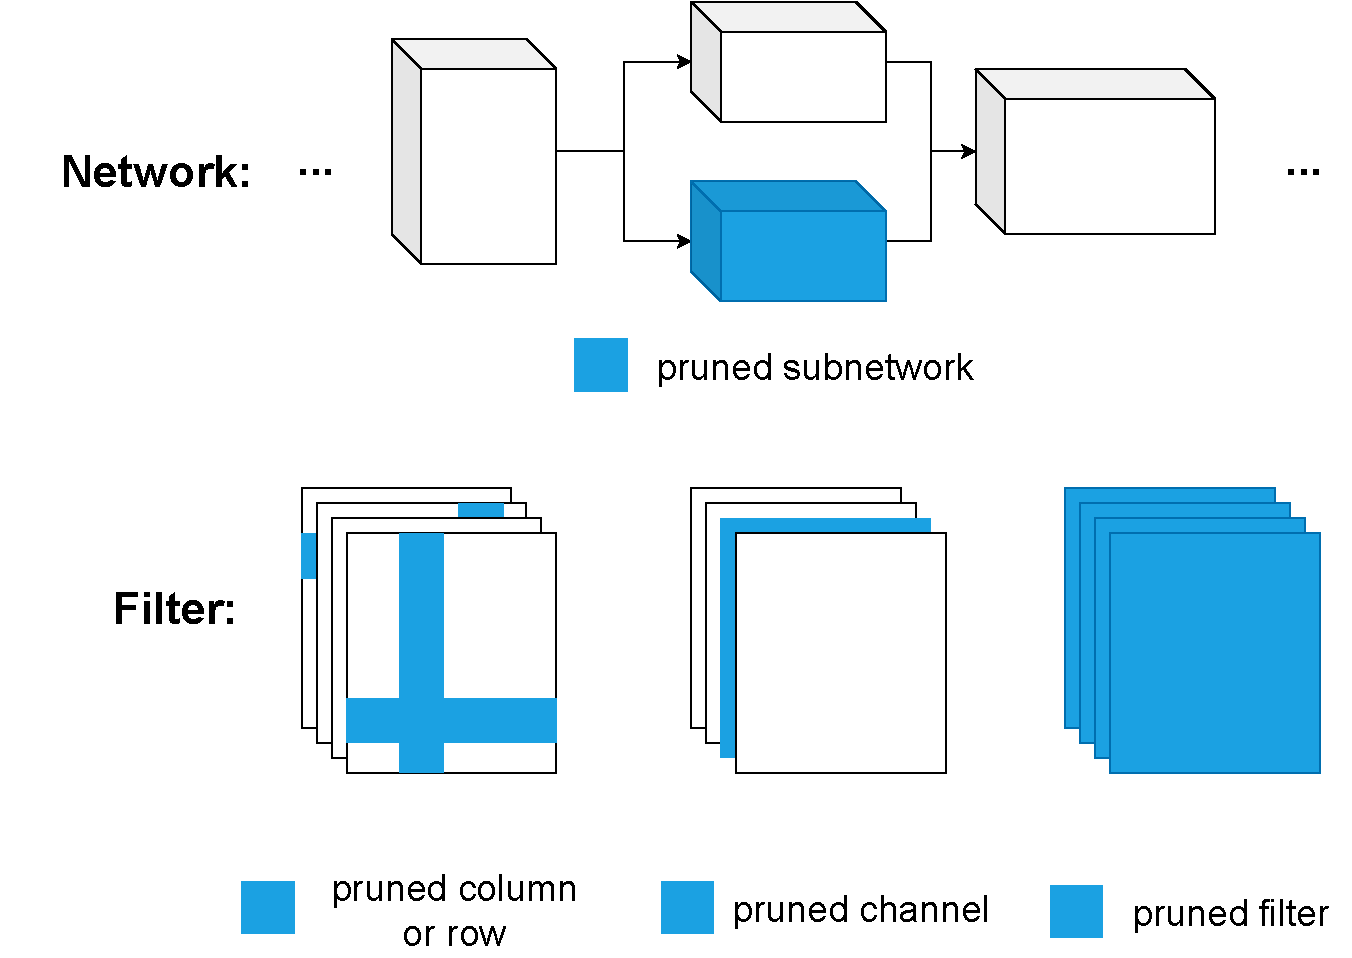
\includegraphics[width=0.6\textwidth]{chapter_sota/assets/structured_pruning.pdf}}
  \hspace{0.09\textwidth}
  \subfloat[Élagage non structuré\label{fig:sota:unstructured_pruning}]{%
    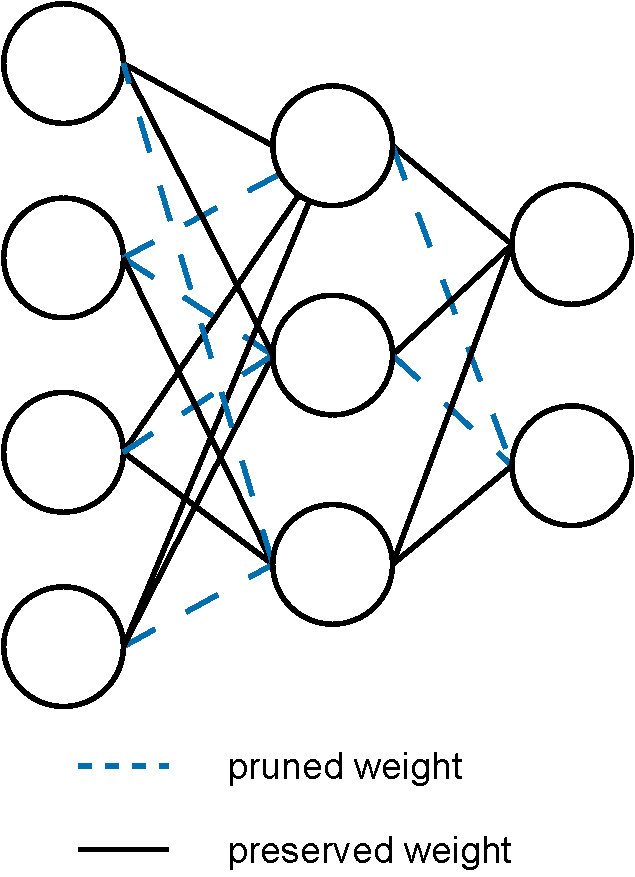
\includegraphics[width=0.3\textwidth]{chapter_sota/assets/unstructured_pruning.pdf}}
  \caption{Illustrations conceptuelles de l'élagage structuré et non structuré.}
  \label{fig:sota:pruning}
\end{figure}

Au sein des diverses méthodes de compression des réseaux neuronaux profonds
présentées, nous choisissons de mettre l'accent sur l'élagage dans le contexte
de la classification d'images supervisée. L'élagage structuré se distingue par
sa flexibilité, notamment son potentiel d'atteindre des taux d'élagage élevés
par rapport à l'élagage non structuré. Plusieurs raisons motivent ce choix : la
création de réseaux légers tout en préservant ou améliorant la performance du
réseau d'origine, la complémentarité avec d'autres techniques de compression et
la possibilité d'appliquer l'élagage à une architecture existante sans nécessité
de la développer de zéro, permettant ainsi de consacrer du temps de recherche et
développement pour d'autres sujets. Cependant, l'élagage présente des défis,
comme l'identification des poids à conserver qui nécessite souvent un
entrainement et un ajustement fin de ceux-ci qui est coûteux en temps et en
ressources. Dans ce qui suit, nous présentons une nouvelle méthode d'élagage
basée sur une reparametrisation des poids et une fonction de coût budgétaire,
évitant l'ajustement fin ainsi qu'une deuxième méthode qui permet d'identifier
les poids pertinents sans même les entraîner, offrant de nouvelles perspectives
de recherche sur l'entrainement des poids.

\section*{Élagage par reparametrisation avec régularisation basée sur le budget}


Cette section traite du défi de l'élagage de grands réseaux de neurones en
limitant la dégradation de leurs performances. La plupart des méthodes d'élagage
existantes dégradent la performance des réseaux neuronaux à cause de l'étape
d'élagage qui retire des poids des réseaux. Par conséquent, une étape coûteuse
d'ajustement fin de ceux-ci est généralement nécessaire pour compenser la perte
de performances. La méthode que nous introduisons dans cette section contourne
ce problème et produit des réseaux élagués légers avec une dégradation minimale
des performances. Ceci est réalisé grâce à une combinaison de reparamétrisation
des poids qui englobe un substitut de la norme $\ell_0$ et une fonction de coût
budgétaire qui oriente la parcimonie du réseau vers un taux d'élagage
prédéfini.\\

L'élagage est une technique permettant d'obtenir des réseaux de neurones légers en
réduisant les paramètres d'un réseau pré-entraîné, évitant la conception d'une
nouvelle architecture. Deux formes d'élagage existent : \textit{(i)} l'élagage
de poids non structuré, qui supprime des poids individuels basés sur leur
importance, et \textit{(ii)} l'élagage structuré qui élimine des sections
entières du réseau.\\

L'élagage non structuré par magnitude est une heuristique reconnue pour évaluer
la saillance des poids, suggérant que les poids les plus faibles peuvent être
retirés avec un impact minime. Cette méthode peut être formalisée par :\\

\begin{equation}
  \mathbf{w}_{\text{élagué}} = p(\mathbf{w}, \alpha) = \mathbf{w} \odot \mathbf{m}_\alpha
\end{equation}\\


\noindent où $p$ représente une fonction d'élagage,  $\mathbf{w}$ les poids
élagués, $\alpha$, le seuil d'élagage, $odot$ le produit de Hadamard et $\mathbf{m}_\alpha$ un masque binaire
défini par :\\

\begin{equation}
  (\mathbf{m}_\alpha)_i = \begin{cases}
    0 & \text{si } |\mathbf{w}_i| \leq \alpha \\
    1 & \text{sinon}
  \end{cases}
\end{equation}\\

L'élagage par magnitude est composé de trois étapes : l'entraînement standard
des poids, l'élagage par magnitude, puis l'ajustement fin des poids restants.
Une variante itérative \cite{DBLP:conf/nips/HanPTD15} de cette méthode existe
également ou les deux dernières étapes sont répétées jusqu'à atteindre un taux
d'élagage souhaité. L'intérêt pour l'élagage non structuré a été renforcé par la
théorie des \textit{Lottery Tickets} \cite{DBLP:conf/iclr/FrankleC19}, qui
suggère l'existence de sous-réseaux performants au sein de grands réseaux,
identifiables par l'élagage par magnitude. Cependant, malgré les avantages, le
coût computationnel, en particulier pour le réglage fin, reste un défi.\\

Notre méthode fait appel à la reparametrisation des poids pour inclure
l'heuristique de l'élagage par magnitude au sein même de l'expression de
ceux-ci. D'autres travaux ont également utilisé la reparametrisation des poids.
Il s'agit méthode où les poids du réseau, appelés \emph{poids apparents}, sont définis
en fonction d'autres \emph{poids latents}. Une reparamétrisation spécifique,
présentée dans \cite{powerprop}, élève un poids à la puissance de $\alpha$
en conservant son signe (voir \cref{eqn:res1:reparam}), créant ainsi une dynamique où les poids les plus
importants augmentent davantage. L'élagage est ensuite effectué sur ces poids
reparamétrisés.\\

\begin{equation}
  \mathbf{\hat{w}} = \mathbf{w} |\mathbf{w}|^{\alpha-1}
  \label{eqn:res1:reparam}
\end{equation}\\


La plupart des techniques de pruning définissent un taux d'élagage après
l'entraînement initial sans prendre en compte le budget de poids final alloué,
ce qui induit une perte de performance après l'élagage. Des travaux ont abordé
ce problème en ajoutant une fonction de perte, combinée à la fonction de coût de
la tâche apprise via un coefficient de pondération $\lambda$ (voir
\cref{eqn:res1:budg_loss}). la Budget-Aware Regularisation (BAR) loss
\cite{lemaire2019structured}, qui effectue un élagage structuré des canaux des
activations. Cette fonction de coût (BAR) est composé de deux parties : l'une
introduisant la parcimonie et l'autre contrôlant le budget.\\

\begin{equation}
  \mathcal{L}_{\text{totale}} = \mathcal{L}_{\text{tâche}} + \lambda \mathcal{L}_{\text{budget}}
  \label{eqn:res1:budg_loss}
\end{equation}\\


ChipNet  \cite{tiwari2021chipnet} est une autre méthode qui inclut une fonction
de coût induisant la parcimonie, appelée \emph{crispness loss}, et une fonction
coût budgétaire. Les auteurs de ChipNet proposent également plusieurs variantes
de budget, dont le budget de canaux, le budget de volume d'activation et le
budget de paramètres. Après le pruning, les réseaux suibissent un ajustement fin
avec les mêmes hyperparamètres que l'entraînement initial, doublant ainsi le
temps d'entraînement.\\

Pour pallier la baisse de performance qui suit l'étape d'élagage, l'ajustement
fin est couramment utilisé. Cependant, il est coûteux en termes de calcul. Des
travaux ont été réalisés pour proposer des méthodes d'élagage qui évitent le
besoin d'ajustement fin. L'une de ces méthodes, appelée \emph{Optimal Brain
  Surgeon} \cite{DBLP:conf/icnn/HassibiSW93}, utilise la matrice Hessienne de la
fonction de perte pour identifier les poids dont le retrait aura un impact
minimal sur la fonction de coût d'une part, et pour corriger les poids restants
d'autre part. Elle est basée sur l'expression de la fonction de perte à un
minimum local comme suit, avec $\mathbf{H}$ la Hessienne :\\

\begin{equation}
  \delta \mathcal{L} \approx \frac{1}{2} \delta \mathbf{w}^T \cdot \mathbf{H} \cdot \delta \mathbf{w}
\end{equation}\\

Cette méthode est efficace sur de petits réseaux, mais est moins adaptée aux
grands réseaux en raison du coût de calcul de la matrice Hessienne. D'autre
travaux ont développé une approche qui ne necessite pas de calculer la
Hessienne. En particulier,  Kang et al. \cite{DBLP:conf/ijcai/HeKDFY18} ont
proposé une méthode qui introduit la parcimonie pendant l'entrainement du
réseau. La méthode introduite élague les canaux dont la sortie sera nulle ou
négative et qui sera donc rendu nulle par l'activation \ac{ReLU}. L'un des
avantages majeurs de cette méthode est que le réseau n'a pas besoin d'un
ajustement fin supplémentaire après l'élagage. Cependant, bien que ces méthodes
visent à retirer des poids ou des groupes de poids redondants, elles abordent
souvent l'élagage comme une réflexion après coup, ne prenant pas en compte leur
nombre final, ce qui peut entraîner une perte de performance.\\

Pour répondre aux défis de l'affinage fin coûteux et de la prise en compte du
budget final et de la topologie du réseau, nous proposons une nouvelle
reparamétrisation des poids couplée à une fonction de coût budgétaire, le tout,
appuyé sur une norme $\ell_0$ de sustitution. Cette approche apprend à la fois
les poids et la structure d'un réseau allégé. Elle permet une élagage non
structuré tout en contrôlant le nombre de poids non nuls. Testée sur différentes
tâches de classification, cette méthode s'est avérée efficace sans nécessité
d'affinage.\\

Dans ce qui suit, pour une simplicité conceptuelle, nous adopterons une approche
conventionnelle où les entrées des tenseurs multidimensionnels sont indexées par
$i$, en plus de l'indice de couche $\ell$, vectorisant ainsi ces entités pour
faciliter leur manipulation.\\

\subsection*{Principe de la méthode d'élaguage}

La méthode que nous proposons est la combinaison d'une fonction de coût
budgétaire donc l'objectif est de pousser les réseau à respecter un budget en
terme de nombre de poids, ainsi qu'une reparamétrisation des poids qui permet
d'inclure l'apriori de l'élagage par magnitude dans l'expression des poids. Ces
deux composantes  dépendent d'une fonction de reparametrisation $h$ qui joue le
rôle de norme $\ell_0$ de substitution dérivable.\\

La fonction de reparamétrisation $h$ est exprimée dans
l'\cref{eqn:res1:stable_h_expression}. Cette formlation permet de garantir 4 propriétés
essentielles pour cette fonction qui sont :

\begin{itemize}
  \item \emph{Image contrainte}. Nous voulons que l'image de $\mathds{R}$ soit
        le segment $[0, 1]$. Cela permet de s'assurer que les poids reparamétrisés ne
        voient pas leur magnitude augmenter à cause de la reparametrisation.
  \item \emph{Dérivabilité}. Afin de pouvoir utiliser la descente de gradient,
        il faut que la fonction de reparametrisation soit dérivable.
  \item \emph{Symétrie}. La fonction de reparametrisation doit être symétrique
        pour ne pas favoriser les poids positifs ou négatifs.
  \item \emph{Segment borné}. Il doit être possible de borner l'image de
        n'importe quel segment $[-a, a]$ de $\mathds{R}$, par une constance arbitraire
        $\epsilon$, afin de garantir que l'image d'un poid faible par la fonction de
        reparametrisation est un poids faible.
\end{itemize}

\noindent La formulation choisie pour $h$ est donc la suivante :

\begin{equation}
  \label{eqn:res1:stable_h_expression}
  h_t(x) = C_1 \biggl( \text{exp} \bigg\{-\displaystyle\frac{1}{(tx)^n +1}\bigg\} - C_2 \biggr),
\end{equation}

\noindent avec $C_1=\frac{1}{1-e^{-1}}$, $C_2 = e^{-1}$, $t$ un paramètre de
température et $n$ un exposant fixé à 4 dans nos expériences. Cette fonction
vérifie les 4 propriétés définies plus haut et est spécifiquement conçue pour
être stable numériquement, même pour des petites valeurs de $x$.\\

cette fonction de reparametrisation est utilisée dans la définition de nos poids
\emph{apparents} afin de rendre les poids faibles encore plus faible mais de ne
pas modifier les poids forts. La définition de ces poids apparents est donnée
comme suit :

\begin{equation}
  \label{eqn:res1:reparametrized_weights}
  \hat{\mathbf{w}} = \mathbf{w} \odot h_t(\mathbf{w})
\end{equation}\\

La fonction de coût budgétaire s'appuie sur cette fonction de reparametrisation
pour compter le nombre de poids non nuls dans le réseau. Elle est de forme
quadratique afin de faciliter l'optimisation et d'assurer un respect du budget.
Elle est définie comme suit :

\begin{equation}
  \label{eqn:chap1:real_budget}
  {\cal L}_\text{budget} = \biggl( \displaystyle\frac{C(\{\mathbf{w}_1,\dots, \mathbf{w}_L\}) - C_\text{target}}{C_\text{initial}} \biggr)^2.
\end{equation}\\

\noindent avec :

\begin{equation}
  \label{eqn:chap1:cost_function}
  C(\{\mathbf{w}_1,\dots, \mathbf{w}_L\}) = \displaystyle \sum_{\ell=1}^{L} \sum_{i=1}^{\nu_\ell} h_t(\mathbf{w}_{\ell i}).
\end{equation} \\

\noindent où $L$ est le nombre de couches du réseau, $\nu_\ell$ le nombre de
poids de la couche $\ell$, $C_\text{target}$ le budget cible et
$C_\text{initial}$ le budget initial.\\

\subsection*{Expériences}

Afin de valider notre méthode et ses composantes, nous l'avons comparé à
d'autres méthodes ou variantes dans différents cas de figure pour montrer
expérimentalement leurs pertinence.\\

Nous avons comparé notre méthode à l'élagage par magnitude avec et sans
ajustement fin post-entraînement pour différent taux d'élagage. Les résultats
démontrent de meilleures performances pour notre méthode, même comparé à
l'élaguage avec ajustement fin, alors que notre méthode ne nécessite pas cet
ajustement et n'a subit aucun réentrainement des poids après l'élagage. La
\cref{fig:chap1:reparam_vs_mpft_conv4} montre les résultats comparatifs sur les
base de donnée CIFAR-10 et 100 \cite{CIFARdataset} pour un réseau Conv4
\cite{DBLP:conf/iclr/FrankleC19}.\\


\begin{figure}
  \centering
  \subfloat[Conv4 - CIFAR-10]{
    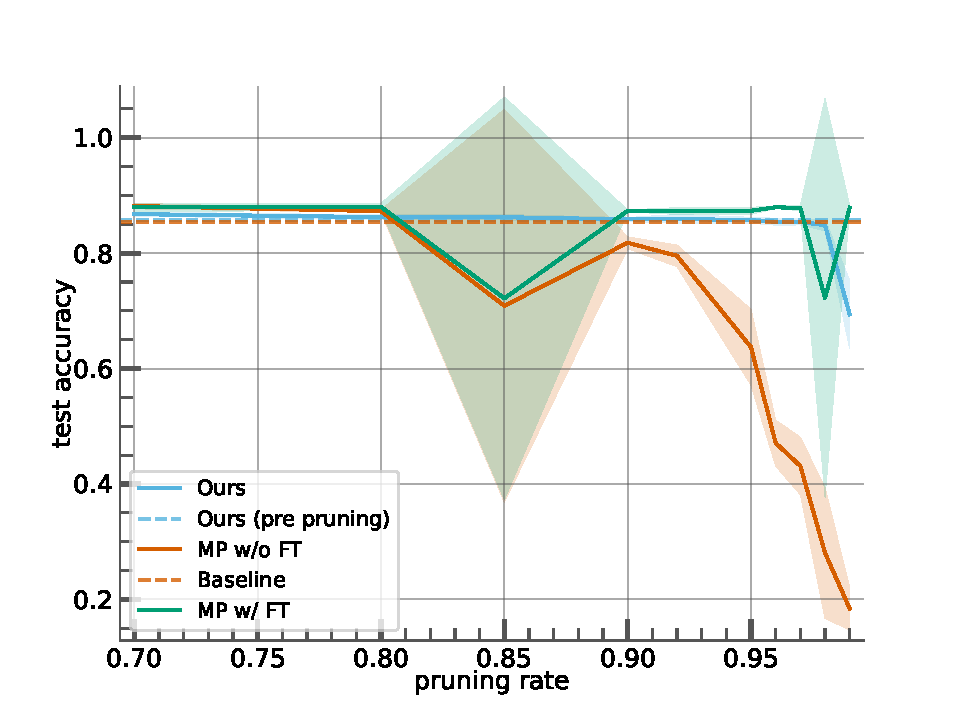
\includegraphics[width=0.49\linewidth]{chapter_1/assets/reparam_vs_mpft_Conv4_cifar10.pdf}
    \label{fig:chap1:reparam_vs_mpft_conv4_cifar10}}
  \subfloat[Conv4 - CIFAR-100]{
    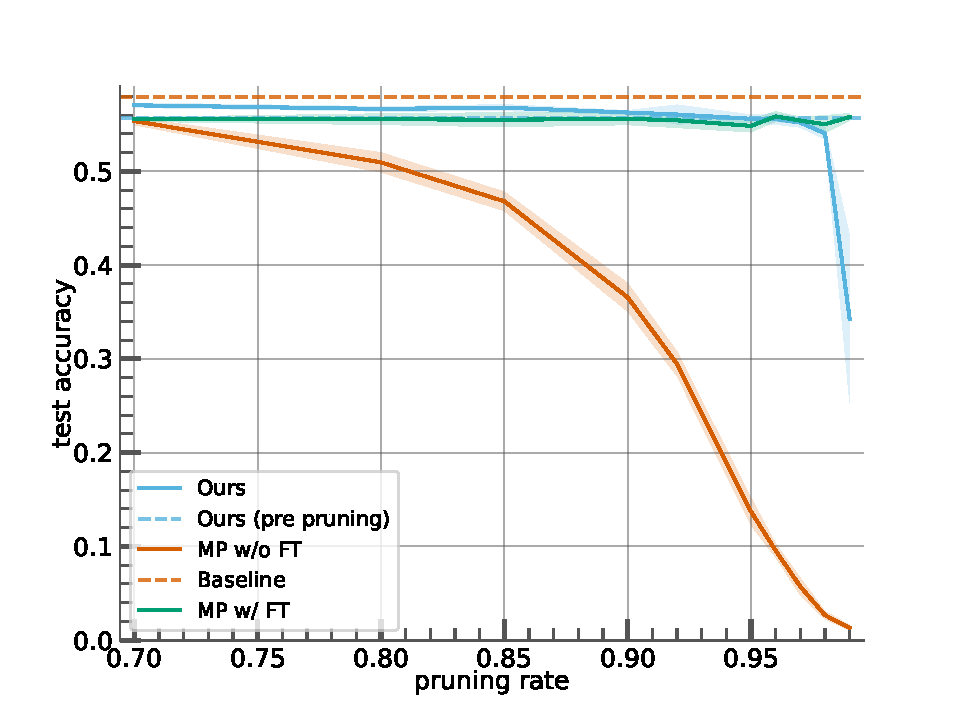
\includegraphics[width=0.49\linewidth]{chapter_1/assets/reparam_vs_mpft_Conv4_cifar100.pdf}
    \label{fig:chap1:reparam_vs_mpft_conv4_cifar100}} \caption{ Comparaison des
    performances de notre méthode {\em(Ours)} face à l'élagage par magnitude
    sans {\em(MP w/o FT)} et avec ajustement fin {\em(MP w/ FT)} utilisant un
    réseau Conv4 sur les ensembles de données CIFAR-10 et CIFAR-100, pour
    différents taux d'élagage. A voir en couleur de préférence.}
  \label{fig:chap1:reparam_vs_mpft_conv4}
\end{figure}

Pour valider l'efficacité de la fonction de coût budgétaire, nous avons comparé
les performances de notre méthode avec deux vairantes. Dans la première
vériante, la fonction de coût budgétaire est simplement retirée de la fonction
de coût global, et dans la deuxième variante, elle est remplacée par
régularisation $\ell_1$ sur les poids du réseau afin d'introduire de la
parcimonie. Nos résultats montrent que notre méthode performe systématiquement
mieux que la variante sans fonction de coût budgétaire et que la variante avec
régularisation $\ell_1$ (à l'exception de l'architecture ResNet-20
\cite{DBLP:conf/cvpr/HeZRS16} pour cette dernière). Il est important que la
variante avec régularisation $\ell_1$ dépend fortement du coefficient de
pondération $\lambda$ (voir \cref{eqn:res1:budg_loss}) et que la valeur optimale
pour $\lambda$ dépend de l'architecture et du jeu de donnée, alors que ça n'est
pas le cas pour notre méthode.\\

Nous avons également validé la fonction de reparametrisation en comparant notre
méthode avec une variante où la fonction de reparametrisation n'est pas
appliquée. Encore une fois, notre méthode performe significativement mieux que
la variante sans reparametrisation une fois que celle ci est élaguée au taux
cible.\\

Ces expériences montrent la pertinence des deux composantes de notre méthode
ainsi que son efficacité comparé aux méthodes d'élagague par magnitude qui
nécessitent un ajustement fin post-entraînement.\\

\subsection*{Points Clefs}

Nous avons introduit une méthode d'élagage des réseaux neuronaux qui surmonte
les limites des méthodes d'élagage traditionnelles. Ces dernières élaguent
généralement les réseaux après une phase d'entraînement initiale sans considérer
le taux d'élagage cible, nécessitant souvent un ajustement fin pour compenser la
perte de précision. En revanche, notre méthode élimine le besoin d'ajustement
fin tout en surpassant les méthodes d'élagage par magnitude actuelles. Elle
s'appuie sur deux composants clés : une fonction de coût budgétaire et une
reparamétrisation des poids. L'utilisation combinée de ces éléments augmente la
robustesse du réseau à l'élagage. Toutefois, la méthode actuelle présente des
limites, notamment l'incapacité de traiter les poids ayant des valeurs identques
ou similaires différemment. Le chapitre suivant introduira une approche pour
déterminer la topologie optimale d'un réseau sans entraîner les poids, en se
basant sur un masque entrainé plutôt que sur la magnitude des poids.\\


\section*{Entrainement de masques pour échantillonnage stochastique des poids}

Dans cette section, nous explorons comment extraire des sous-réseaux performants
et légers de grands réseaux de neurones sans entraîner les poids. Au lieu de se
baser sur la valeur des poids pour établir leur pertinence au sein de
l'architecture, comme dans le chapitre précédent, cette méthode se base sur un
l'entraînement de masques latents. Dans cette méthode, le critère d'élagage
n'est plus lié à la valeur du poids et l'on se concentre sur la sélection de la
topologie plutôt que sur l'entraînement de ces derniers. Cette approche est
adaptée pour des situations où modifier les poids n'est pas possible et offre
une nouvelle perspective à l'entraînement des réseaux de neurones en s'éloignant
du paradigme qui consiste à entraîner les poids.\\

Certains travaux se sont attaqué au problème de l'élagage en adoptant une
approche consistant à élager les poids du réseau avant l'entraînement de
ceux-ci, c'est à dire à leur initialisation. C'est le cas notamment des méthodes
SNIP \cite{DBLP:conf/iclr/LeeAT19}, GraSP \cite{DBLP:conf/iclr/WangZG20} and
SynFlow \cite{DBLP:conf/nips/TanakaKYG20}. Ces 3 méthodes établissent chacune un
critère de pertinence des poids dérivé de leur valeur et élaguent les poids
avant même l'entrainement de ceux-ci. Il reste tout de même nécessaire de faire
quelques passes d'entrainement pour calculer les critères de pertinences, et un
entraînement complet des poids restants reste nécessaire.\\

L'élagage à l'initialisation des poids, peut-être vu comme une manière de
chercher un sous-réseau performant au sein d'un réseau plus grand. C'est cette
problématique particulière qu'ont choisit d'aborder Frankle et al.
\cite{DBLP:conf/iclr/FrankleC19} avec leur méthode des \emph{Lottery Tickets}.
Pour trouver un sous réseau performant \emph{après entrainement}, les auteurs
entraine d'abord un grand réseau, puis élagent les poids par magnitude et
restaurent les poids restants à leur valeur initiale. Le sous réseau alors
obtenu est appelé \emph{Lottery Ticket} et performe aussi bien que le grand
réseau lorsqu'entraîné. Cette méthode a été étendue à des réseaux plus
profondset plus grand en adaptant la procédure pour que  l'élagage soit
iteratif, et les poids restorés non pas à leur valeur d'origine mais à une
valeur postérieur à l'initialisation \cite{DBLP:conf/icml/FrankleD0C20}. Ces
travaux ont été précisés dans \cite{DBLP:conf/iclr/LiuSZHD19}, où les auteurs
montrent que seul la topologie est importante et pas la valeur des poids.\\

Si Frankle et al. ont montré que l'on pouvait extraire un sous réseau performant
une fois celui-ci entrainé, il existe un sous réseau performant sans même avoir
besoin de l'entrainer. Ce résultat a d'abord été conjecturé dans
\cite{DBLP:conf/cvpr/RamanujanWKFR20} en tant que \emph{Strong Lottery Ticket
Hypothesis} (Hypothèse forte du billet de lotterie). Des démonstration formelles
ont été proposée et prouvent l'existence de ces sous réseau avec des conditions
sur la taille du réseau d'origine
\cite{DBLP:conf/icml/MalachYSS20,DBLP:conf/nips/OrseauHR20,DBLP:conf/nips/PensiaRNVP20}.
Ces preuves cependant ne sont pas constructives et ne donnent pas de méthode
pour trouver ces sous réseaux. Des travaux ont proposé des heuristiques basées
sur des masques binaires pour trouver ces sous réseaux
\cite{DBLP:conf/nips/ZhouLLY19} ou bien via l'entrainement de variables
auxiliaires seuillées \cite{DBLP:conf/cvpr/RamanujanWKFR20}.



\subsection*{Principe de la méthode d'élagage}

Notre méthode est basée sur deux composantes principales. La première étant une
technique d'échantillonnage stochastique des masques, et la deuxième étant un
mécanisme de mise à l'échelle des distributions de poids. \\

La première composante permet l'entrainement de masques qui déterminent la
saillance (c'est à dire la pertinence) des poids du réseau. Cette saillance est
interprété dans notre méthode comme la parametrisation de la probabilité pour le
poid d'être conservé. Grâce à ces probabilités, on peut échantillonner des
topologies, les évaluer et ajuster les probabilités en conséquence. On souhaite
entrainer des masques via la méthode classique de la descente de gradient.
Cependant, l'opération d'échantillonnage n'est pas dérivable. Nous proposons
donc la méthode \ac{ASLP} (log-parametrisation décallée arbitrairement). Cette
méthode d'échantillonnage permet d'entraîner les masques avec des méthodes de
gradient. Cette méthode est basée sur \ac{STGS} qui considère les
log-probabilités des différents évènements. Dans notre cas nous considérons deux
évènements : la conservation du poids et son élagage. Le vecteur de log
probabilité des deux évènements pour une connection entre les neurones $i$ et
$j$ s'écrit comme suit :

\begin{equation}
  \label{eqn:chap2:log_prob}
  \log(\mathcal{P}_{ij}) = \begin{bmatrix}
    \log(p^\text{conserver}_{ij}) \\
    \log(p^\text{élaguer}_{ij})
  \end{bmatrix}
\end{equation}

\noindent Les deux évènements étant mutuellement exclusifs, nous réécrivons
$p^\text{conserver}_{ij} = p_{ij}$ et $p^\text{élaguer}_{ij} = 1 - p_{ij}$. De
plus, nous considérons que $p_{ij}$ est parametrisé par un masque latent
$\hat{m}_{ij}$ comme suit:

\begin{equation}
  \label{eqn:chap2:prob_param}
  p_{ij} = \frac{1}{1 + \exp(-\hat{m}_{ij})} = \sigma(\hat{m}_{ij})
\end{equation}

\noindent où $\sigma$ est la fonction sigmoïde. Le vecteur de log probabilité
s'écrit donc :

\begin{equation}
  \label{eqn:chap2:log_prob_param}
  \log(\mathcal{P}_{ij}) = \begin{bmatrix}
    \log(\sigma(\hat{m}_{ij})) \\
    \log(1 - \sigma(\hat{m}_{ij}))
  \end{bmatrix}
\end{equation}

Cependant, cette formulation est complexe, coûteuse en calcul et peu stable
numériquement à cause de la composition des fonctions et sigmoïde (elle même
composée de fonctions exponentielles). Nous proposons donc une formulation plus
simple d'une part et stable numériquement d'autre part. Nous définissons le
vecteur de log probabilité comme suit :

\begin{equation}
  \label{eqn:chap2:log_prob_param_simple}
  \log(\mathcal{P}_{ij}) +\begin{bmatrix}
    c \\
    c
  \end{bmatrix} = \begin{bmatrix}
    \hat{m}_{ij} \\
    0
  \end{bmatrix}
\end{equation}

\noindent La partie droite de l'\cref{eqn:chap2:log_prob_param_simple} garantie
que la probabilité $p_{ij}$ est toujours paramétrisée de la même façon,
c'est-à-dire par $\sigma(\hat{m}_{ij})$, mais représente le vecteur de log
probabilité de l'\cref{eqn:chap2:log_prob_param} à une $c$ près inconnue. C'est
cette constante qui donne son nom à la méthode. L'utilisation d'une constante ne
change pas les résultats du \ac{STGS} car celui-ci utilise un argmax qui n'est
pas affecté par le décallage induit par la constante $c$. C'est donc le vecteur
de droite de l'\cref{eqn:chap2:log_prob_param_simple} qui est utilisée en lieu
et place du vecteur de log probabilité pour l'échantillonnage des masques avec
\ac{STGS}.\\

La deuxième composante de notre méthode est un mécanisme de mise à l'échelle des
distributions de poids. L'élagage des poids introduit par l'échantillonnage des
masques perturbe les statistiques des distributions de poids de chaque couche du
réseau. Ceux-ci n'étant pas entrainé, il est important de conserver les bonnes
statistiques pour une bonne propagation du gradient
\cite{DBLP:conf/iccv/HeZRS15}. Nous proposons donc un mécanisme de mise à
l'échelle des distributions de poids. Ce mécanisme est basé sur la
multiplication avec un paramètre apris. Pour chaque couche $\ell$ du réseau,
nous multiplions les poids par un paramètre appris $s_\ell$. Cette méthode est
plus rapide et moins couteuse en calcul que les méthodes de mise à l'échelle
précédentes qui se basent sur le calcul explicite du taux d'élagage dans chaque
couche \cite{DBLP:conf/cvpr/RamanujanWKFR20,DBLP:conf/nips/ZhouLLY19}.

\subsection*{Expériences}
Afin de valider notre méthode et ses composantes, nous l’avons comparé à
d’autres méthodes ou variantes dans différents cas de figure pour montrer ex-
périmentalement leurs pertinence.\\

Pour valider le mécanisme de mise à l’échelle des distributions de poids, nous
l'avons comparé à une variante sans mise à l'échelle et également aux autres
méthodes de mise à l'échelle des distributions de poids. Il ressort de nos
expériences que notre méthode de mise à l'échelle des distributions de poids
permet de conserver les bonnes statistiques de poids et est plus rapide et moins
couteux en calcul que les autres méthodes. De plus, notre méthode permet une
réduction du nombre d'époques requises pour l'entrainement, ainsi qu'une
amélioration des performances.\\

Le taux d'apprentissage \emph{(learning rate)} que nous avons utilisé est de 50,
ce qui est une valeur élevée au regard des méthodes d'entrainement classiques.
Nous avons conduit une série d'expériences pour juger de l'impact du learning
rate sur notre méthode et de la valeur optimale à choisir. Il en ressort d'une
part que notre méthode d'entrainement des masques est robuste aux variations
extrèmes du taux d'apprentissage car il est possible de l'entraîner avec des
valeurs de 500 ou plus sans observer d'instabilité numérique. De manière
remarquable, même un taux d'apprentissage de 50 permet d'obtenir des résultats
convaincant. D'autre part nous avons observé que la diminution du taux
d'apprentissage en cours d'entraînement n'avait pas d'effet, et nous avons pu
valider le choix de 50 pour la valeur du taux d'apprentissage. Il s'agit de la
valeur qui donne le meilleur compromis entre performance finales et temps
d'entraînement.\\

La topologie des réseaux  entraîné par notre méthode étant stochastique, nous
avons choisi de la fixer pour pouvoir évaluer les performances de notre méthode
sur les jeux de données d'entraînement. Pour ce faire nous gardons tous les
poids qui ont une probabilité de selection supérieure ou égale à 0.5 et élaguons
tous les autres. Nous avons pu montrer expérimentatlement que cette façon de
faire donne de meilleures performances que la méthode de moyennage utilisée par
les travaux précédents \cite{DBLP:conf/nips/ZhouLLY19}. De plus, nous avons mis
en évidence la robustesse de notre méthode a une élévation du taux d'élagage une
fois le réseau entraîné. Il nous a été possible d'augmenter celui-ci de près de
30 points perte de performance notable.\\

Enfin, nous avons comparré notre méthode à d'autres méthodes d'élagage sans
entrainement des poids de l'état de l'art via un jeu d'expériences reproduisant
de nombreuses configurations testées par les auteurs de ces méthodes (Edge Popup
\cite{DBLP:conf/cvpr/RamanujanWKFR20} et Supermask
\cite{DBLP:conf/nips/ZhouLLY19}). Nos résultats ont démontré la supériorité de
notre méthode en terme de performance sur les jeux de données d'entraînement
dans la totalité des scénarios testés et ce pour la quasi majorité des
architecture et jeux de données considérés. La table \cref{tab:res2:r20_VGG16_performances_comparison}\\

\begin{table}[htbp]
  \centering\begin{tabular}{llcc}
    \cmidrule[\heavyrulewidth]{3-4}
                                                          &                                                  & \multicolumn{2}{c}{\textbf{Dataset}}                             \\
                                                          &                                                  & \textbf{CIFAR-10}                    & \textbf{CIFAR-100}        \\
    \toprule
    \multirow{6}{*}{} \multirow{4}{*}{\textbf{ResNet-20}} & \ac{ASLP} (thresholding)                              & \textbf{ 81.08 $\pm$ 0.50}           & \textbf{44.63 $\pm$ 0.91} \\
                                                          & \ac{ASLP} (averaging)                                 & 78.85 $\pm$ 0.41                     & 42.91 $\pm$ 1.14          \\
                                                          & \cite{DBLP:conf/nips/ZhouLLY19} (averaging)      & 69.83 $\pm$ 1.20                     & 30.60 $\pm$ 0.91          \\
                                                          & \cite{DBLP:conf/cvpr/RamanujanWKFR20} ($k=50\%$) & 75.09 $\pm$ 1.41                     & 22.47 $\pm$ 1.37          \\
    \midrule
    \multirow{4}{*}{\textbf{VGG16}}                       & \ac{ASLP} (thresholding)                              & \textbf{24.93 $\pm$ 0.69}            & \textbf{8.66 $\pm$ 0.33}  \\
                                                          & \ac{ASLP} (averaging)                                 & 24.93 $\pm$ 0.77                     & 8.58 $\pm$ 0.32           \\
                                                          & \cite{DBLP:conf/nips/ZhouLLY19} (averaging)      & 25.07 $\pm$ 0.34                     & 7.97 $\pm$ 0.35           \\
                                                          & \cite{DBLP:conf/cvpr/RamanujanWKFR20} ($k=50\%$) & 23.05 $\pm$ 0.84                     & 6.65 $\pm$ 0.38           \\
    \bottomrule
  \end{tabular}
  \caption{Comparaison de la \textbf{précision de test} d'\ac{ASLP} par rapport
  à Edge-Popup et Supermask
  \cite{DBLP:conf/cvpr/RamanujanWKFR20,DBLP:conf/nips/ZhouLLY19} sur les bases
  de données \textbf{CIFAR-10} et \textbf{CIFAR-100} en utilisant les
  architectures VGG16 et ResNet-20. Les résultats présentent le scénario avec
  augmentation de données, \acf{WR} et distribution de poids \acf{SC}. Sur
  l'ensemble des bases de données et des architectures de réseau, \ac{ASLP}
  dépasse les méthodes comparatives dans sa configuration de
  \textit{thresholding} qui correspond à notre méthode de fixation de la
  topologie. }
  \label{tab:res2:r20_VGG16_performances_comparison}
\end{table}


\subsection*{Points Clefs}

Nous avons introduit une méthode d'entrainement d'élagage de réseaux de neurones
qui ne repose pas sur l'entrainement des poids mais bien sur celui de masques
latent qui déterminent les probabilités de selection de ces poids. Cette méthode
permet de procéder à la selection de la topologie la plus optimale pour un jeu
de poid donné et fixés. Elle est basée sur deux composantes principales : une
méthode d'échantillonnage des poids tirant profit d'une formulation simple et
numériquement stable du vecteur de log-probabilité, ainsi que d'un mécanisme
rapide de mise à l'échelle des distributions de poids. D'un point de vu général,
cette méthode permet d'extraire un sous réseau performant d'un réseau plus grand
sans en entrainer les poids. Cela permet d'une part d'obtenir des réseaux légers
et d'autre part de jetter un nouvel éclairage sur l'entrainement des réseaux de
neurones en considérant la selection de topologie comme une alternative à
l'optimisation des poids.\\

\section*{Conclusion}

Cette thèse traite de la compression des réseaux de neurones profonds, en se
concentrant sur le problème de la baisse de performance après l'élagage. Nous
avons proposé des solutions pour ce problème et remis en question la nécessité
de former les poids. Deux contributions principales sont présentées : d'abord,
une méthode d'élagage respectueuse du budget avec reparamétrisation du poids,
qui optimise conjointement les poids et la topologie du réseau. Elle a démontré
une performance supérieure à l'élagage basé sur la magnitude dans diverses
expérimentations. Deuxièmement, nous introduisons une méthode d'élagage sans
formation de poids avec échantillonnage stochastique, qui estime l'importance
d'un poids sans se lier à sa valeur, mais par l'optimisation des masques
auxiliaires. Elle a montré de meilleures performances par rapport à d'autres
méthodes de pointe. Notre code est disponible publiquement pour reproduire nos
résultats.

De futures perspectives de recherche pour améliorer les méthodes proposées dans
cette thèse sont possibles.  Nous suggérons d'effectuer une validation
expérimentale sur des ensembles de données et des architectures plus vastes,
permettant une exploration plus approfondie de l'espace de la topologie. Nous
envisageons également l'adoption de l'élagage structuré pour obtenir une
accélération plus directe avec les logiciels et bibliothèques d'apprentissage
profond populaires. Nous proposons des améliorations, telles que le contrôle de
l'ampleur du masque, l'adoption d'un meilleur schéma d'initialisation pour la
méthode \ac{ASLP}, et l'exploration de la possibilité d'entraîner un réseau par
l'élagage sans entraîner les poids. Ces idées orientent les recherches futures
pour optimiser les techniques d'élagage des réseaux neuronaux.




\newpage

%récupérer les citation avec "/footnotemark" \nocite{*} -> nocite fait que tout
%les éléments sont cités même s'ils ne sont pas dans le texte de base. Ici, on
%veut juste les citations qui sont dans le corps du résumé.

%choix du style de la biblio
\bibliographystyle{plainnat}
%ajout de la bibliographie dans la table des matières
\addcontentsline{toc}{chapter}{Bibliography}
%inclusion de la biblio
\bibliography{bibliography.bib}
%voir wiki pour plus d'information sur la syntaxe des entrées d'une bibliographie


\end{document}